
\chapter{Dravidianism with Language Equaling Race – The Third Wheel in Tamil-Sanskrit Interactions}

\Authorline{Ravi Joshi and Yamuna Harshavardhana}


\section{Abstract}

This paper will attempt to collect the strands of Western Oriental scholarship specific to the linguistic and race-based colonial era hypotheses, which led to the establishment of the heavily racialized political atmosphere in Tamil Nadu of the past hundred or so years. It will also investigate why this polarized thinking worked especially well in Tamil Nadu, as opposed to the neighboring states of Kerala, Karnataka and Andhra/Telangana. It will rely on the baseline laid down in books like "Breaking India - Western Interventions in Dravidian and Dalit Faultlines", and attempt to further flesh out the academic background that answers some of these questions. The theories on which this scholarship has been built will be problematized. Also questioned will be the lack of responsibility of the scholars – for example Romila Thapar and others of the Marxist School of Indian History – who should know how politicized theories take a life of their own, often solidifying into rigid dogmas long after the underlying premises themselves of these theories have been shown to be false.


\section{Introduction}

The trope of Dravidianism, which owes its roots to the 18th century discovery of the Dravidian family of languages, has deep ramifications for colonial and post colonial India, continuing upto the present. This in turn was based on Indological scholarship which held the Biblical idea of “Language equals Nation” as a founding axiom, although this was not always clearly spelt out in the scholarship. This idea drew upon notions of the mythical Noah’s sons populating the world with various ‘nations’ and peoples’ who took the original languages from the “Tower of Babel”. A one-to-one correspondence between languages and nations/people as its carriers was assumed. Introduced initially into scholarship via the intense gaze and studies of Christian missionaries and their motivated conclusions, its legitimacy was fully established via the erstwhile Madras School of Orientalism which produced the “Dravidian Proof” c.f. Trautman. It further got installed downstream as common wisdom especially with the advent of English education in Tamil Nadu. Initially, it was people like German Missionary Friedrich Schwartz (Frykenberg 2008:152-165) who started English medium schools that catered mostly to elites in the Tinnevely (Tirunelveli) area. This model was subsequently replicated in stages all over India. The subsequent complete Macaulayite revamp of the Indian education system made its legitimacy virtually uncontested, where elite, both intellectual and political, were fed the Nouveau Orientalist idea – hatched in the “language mills of Madras Fort St George” c.f. Trautman.

The ruling historical paradigm was of an India of ‘indigenous Dravidians’ conquered by Sanskrit bearing Aryans who either pushed all ‘Dravidians’ into the lower rungs of the “Caste system”, or created sub-human “Dalits” or “\textit{Adivasi}s”\index{Adivasi} outside the pale of ‘civil society’, forcing them into conditions worse than those of historical slavery. The establishment of the South Indian Dravidian family of languages as a language family independent of the “Aryan” (subsequently “Indo-European”) Sanskrit based language family was the first step, and this construct burst through the bounds of legitimate linguistic studies to – immediately and automatically – take on racial overtones. The work of Trautman traces the Bible based genesis of the idea of language = nation (now “Race”), and how this axiomatic construct is even now a relatively unexamined axiom of linguistic studies, and how it was used globally to study ‘origins’ of languages and ‘peoples’. While this may be only of academic interest elsewhere, for the living civilization of India, this has deep implications for how the divisive rhetoric of Dravidianism has worked in the realm of social relations and geopolitics. The book “Breaking India” (Malhotra 2011) has covered this in extensive detail. In this paper the intent has been to see how this new categorization, after using the useful structures from sophisticated Indic linguistic science, completely subsumed it to produce radically new constructs of a “Racially” divided India from pre-historic times. Needless to say, Indian linguistics atrophied after this, since the ‘essence’ was sucked out and ‘preserved’ in the more ‘modern’ and ‘scientific’ western linguistics.

This process had both a religious and a secular component which went hand in hand.Tracking its path through stages shows that initially it was Christian missionaries – operating mainly in and around the deep south coastline of India between Madras \& Cochin – that spread these western memes of an incongruous coupling of Christian Gospel with Enlightenment equated to scientific-technological sensibilities. This narrative of Progress was energetically sold to the local populace and yielded converts, especially amongst the aspirational underclass. Along with this went the idea of creating a sense of grievance against specific traditional elites which encouraged appeals and petitions by this underclass to the current ruling dispensation, i.e. the Colonialists. This was followed by almost a century where their institution and alliance-building groundwork promoted these ideas which became ground realities in the ‘subaltern’ sections of society. These new institutions also mobilized converted people and put the ruling dispensation – local Nawabs and Maharajas, as well as the East India Co. succeeded later by the British crown – on notice. The loud and clear message was that they and their interests were a force to be reckoned with, in any Colonial ruling mechanism. One can also see that independent India’s continuance of most Colonial governance structures under the name of Liberal Parliamentary Democracy – which mostly ignored India’s own past republican/democratic institutions – has only accelerated this trend.

The next stage was in the nominally secular realm of Colonial administrative officials who also often doubled as Orientalists. Here is where path breaking scholars like F W Ellis etc. (Trautman2006: 151-185) came up with their compelling “Dravidian Proof”. A careful blending of insights provided by Indic linguistic science – which provided both hard data \& theoretical knowledge of pan India linkages between Indian languages, and European linguistic practice – which seems to have mainly provided axioms and a teleology, produced an overarching Universalist theory of languages, which became used globally. The Indic languages were decisively split into being parts of two global language ‘families’, the Aryan (later redubbed ‘Indo-European’) family pertaining to North India, and the newly certified Dravidian family, with Tamil as its fount, pertaining to India south of the Vindhya mountains. When the discoveries at the Harappa and Mohenjo-Daro sites came to light, the AIT hypothesis was solidified based on this ‘hard data’ combined with the “Dravidian Proof” of ‘genetic’ separateness from Sanskrit. The conflation of linguistic ‘family separation’ with ‘racial’ separation was actively pursued, though never much mentioned explicitly, let alone problematized. Strenuous efforts were – and still are – made in mainstream scholarship to show that the so-called (Christened?) indigenous ‘Dravidians’ occupied the whole of the subcontinent and beyond – as far as the Middle East. Of late, the Biblically derived idea of ‘language tree’ with one ‘genitive ancestor language/people’ spawning branches etc, is slowly giving way to more realistic hypotheses; of languages as overlapping and porous zones of influence, merely correlating to ‘peoples’ but not indelibly linked to them. But this is yet to have any impact on the theoretical validity of either the idea of a discoverable ‘Proto language’, or the derived Dravidianism as a contentious racial construct. This overall context is well framed by (Chakrabarti 1997: 166-180) with focus on Indus Valley civilization, and by (Inden 2000: 117-130) on the Dravidianization \& consequent decline of the invader ‘Aryan’ mind in hot humid ‘female’ India.

Two Biblically driven core presumptions tying language \& race are, namely the idea of Language Tree with some ‘Ur’ pure language spawning a genetic family, and the closely intertwined idea of ‘humanity’ bursting forth – encoded proto language, culture \& all – from ‘Ur’ ‘source’ locations like the Middle-East – later extended to Europe and Central Asia – to put indelible racial stamps on ‘sink’ locations like India which are stereotypically forever swamped by invaders.

The ‘grey’ in-between area around the Vindhyas and Northern Deccan still has a hard time fitting into these stark dichotomies of Aryan/Dravidian, both in linguistic and racial/ethnic terms. Beyond letting the archaeologically attested Megalithic cultures of prehistory carry the burden of being co-opted as part of a “pre Aryan, Dravidian world”, the Indologists’ dispensation glosses over their ill-fitting appearance in their black and white theories. The Emic views, which were linguistically \& ‘ethnically’ (i.e. with due considerations to \textit{deśa} and \textit{jāti}) fairly robust \& well documented in Indian literature, are totally ignored except as fodder \& mere data to support Indological theory. A properly comprehensive view would mean taking seriously the Indic Emic categorical analysis which has structured categories where formal Sanskrit is related via rules to locally spoken Desha bhasha, Prakrits etc.

Thus the current sociopolitical situation in Tamil Nadu is based on explaining the laudable and traditionally uncontested uniqueness of Tamil using a lens of radical separateness, and then using this to push a divisive agenda that has Dravidianism as one of its prime movers. This is notwithstanding the fact that ‘race’ has long been discredited as a scientific construct and Biblically driven linguistics is also being dethroned from its silent presence in unquestioned axioms of historical linguistics.


\section{(A) MAJOR THEMES}

\subsection{Dravidian Ideology and its Politics}

\subsubsection{1. The Dravidian Premise}

Justice Party was started in the early 20th century as an anti-Brahmin political organisation; it was withdrawn from politics in 1944 and renamed as Draviḍar Kalagam, a social organisation, under the leadership of ‘Periyar’ E. V. Ramasamy. After that, the Draviḍian Parties, the political offshoots of the Draviḍar Kalagam, have held Tamil Nadu in their ideological sway for over half a century.

Despite the long-time attempts of the Dravidianists to bring under their umbrella the other southern states of Kerala, Andhra Pradesh/Telengana and Karnataka, they have not materialised owing to several reasons. Firstly, the name Dravida is held by Southern Brahmins who have a significant presence in Karnataka (along with ‘non-Dravidian’ Maharashtra and Madhya Pradesh). Dravida Brahmins are common in Andhra Pradesh. This name has roots in defining the geographical origin of the Brahmin communities and has nothing to do with race. Since Dravidianism is anti-Brahmin in its very nature, the conflict is apparent. Secondly, Malayalam, Kannada and Telugu languages, though they have a vast vocabulary that are southern in origin, have long adopted the Devanagari phonetic system and alphabet. There is a significant linguistic syncretism between Sanskrit and these languages which is very obvious to the layman. It, therefore, becomes quite challenging to adopt the Dravidianist stance and question Sanskrit. [Note: Despite claims of being distinct, the Tamil alphabet layout is identical to Devanagari with the exceptions that Tamil has a few phonetic distinctions and has no aspirated consonants] Thirdly, the work of the Christian Missionaries in the early years was to show a clear distinction between ‘root’ languages and ‘derived’ languages. Tamil became categorised as a root language while the others are derived languages (notwithstanding the fact that each of these languages has a vast repository of their own vocabulary not found either in Tamil or Sanskrit). This places these languages at a position beneath Tamil as per the Dravidianist thought which, naturally, will not be savoured by the political setting of the states. These reasons are way too obvious and are not wishful surmises. Hence, we shall deal with Dravidianism, especially its politically motivated avatar, seen exclusively in Tamil Nadu.

This section aims to uncover the basis of the lingual, ethnic, irreligious, parochial, casteist and divisive ideologies propagated by Draviḍar Kalagam and the Draviḍian parties. E. V. Ramasamy repeatedly quotes Caldwell and endorsed the Aryan Invasion Theory in his speeches and writings.

\begin{myquote}
We do not need to explain how theAryansentered and settled in the Dravidian country, and subjugated and oppressed the Dravidians. Nor do we need to explain how before the Aryans entered the Dravidian country, the Dravidian country had a civilization and arts of the highest rank.
\end{myquote}


~\hfill - Viduthalai 07-09-1953

He further says,

\begin{myquote}
Aryan culture is different ours is different. Aryans are different we are different. Ariyam is different – Draviḍam is different. These feelings and thoughts are seen among people only in the past 50 years, and that too in very few people only.
\end{myquote}


~\hfill - Viḍutalai 03-09-1956

The above, though an attempt to reinforce the Aryan-Dravidian divide,\index{Aryan-Dravidian divide} endorses that the very notion of Aryan-Dravidian divide began a mere half-century earlier (at that time).


\subsubsection{2. The Aryan Invasion Theory (AIT)}

The AIT has not found scientific traction based on either archeological, genetic or literary hard data. First, there is no physical evidence of an invasion followed by mass annihilation and/or exodus\endnote{This news is on to the unearthing in Hisar of 4 skeletons that are determined to be 5000 years old which will be used for genetic testing. https://bit.ly/1QG6Uos}. Second, there is no evidence to show any form of genetically distinct identities, viz., Aryan and Dravidian, in the subcontinent. India’s population mix has been stable with no evidence of Central Asian gene influx for the past 10,000 years\endnote{Sengupta et al. Polarity and Temporality of High-Resolution Y-Chromosome Distributions in India Identify Both Indigenous and exogenous Expansions and Reveal Minor Genetic Influence of Central Asian Pastoralists. \textit{The American Journal of Human Genetics}, February 2006.}. The Ancestral North Indians (ANI) and the Ancestral South Indians (ASI) can be genetically accounted for only in times earlier than 8000 BCE. Detailed genetic studies have all concluded to there being very limited variations in the population gene-pool both at the linguistic level and at the caste level\endnote{Michel Danino, Genetics and the Aryan Debate, https://bit.ly/2n4Hcz6}.

Third, there is no literary reference to any invasion and subjugation either by the (supposed) invader or by the invaded peoples\endnote{The complete works of Swami Vivekananda, Jan 1989, Vol. V, P 534}. The word Dravida does not appear in the Vedas. This has profound significance because the Vedas and the Vedic people are familiar with battles and proudly refer to several of them. Next, there is zero reference to the areas of the subcontinent from which the Aryans are accused of having pushed away the Dravidians\endnote{Rigveda (Book 7, hymns 18, 33 and 83.4-8) is the Battle of the Ten Kings}. On the other side, the word ‘Aryan’ and several of its variants are seen in the Tamil Sangam literature (dated to have begun in the 3rd century BCE) over several centuries but none of the usages to which the word is subjected to has any racial/cultural implication. This is in stark contrast to the common references to the Bauddhas (Buddhists) and the Samanas (Jains) as distinct (sometimes hostile) religious sects\endnote{https://en.wikipedia.org/wiki/Manimekalai}in these works as well as in inscriptions\endnote{https://bit.ly/2utdZ7o, https://bit.ly/2uwNVsb, https://en.wikipedia.org/wiki/Sittanavasal}. An occurrence of such magnitude as the Aryan Invasion – which is purported to have turned topsy-turvy the social and political equations – is mentioned in none of the earliest Tamil works which is concrete proof that it never occurred in the first place.

Further, there is no reference to any such invasion in any of the literary or oral traditions of the outsiders while referring to the Aryans and the Dravidians.


\subsubsection{3. Context and meanings in the usage of the terms, ‘Aryan’, ‘Dravidian’ and ‘Tamil’ from ancient literature until Colonial times and AIT}

The word ‘Draviḍa’ is conspicuous by its absence in Sangam literature.\index{Sangam literature} It is not seen in any of its variants either such as ‘draviḍar’, ‘draviḍam’ and so on. The word ‘Draviḍa’ itself is not of Tamil origin and can be simply proven by the fact that Tamil grammar\index{Tamil grammar} does not provide for two of the details of the word: First, no word begins with a voiced plosive (here, the dental plosive) and so cannot begin with ‘d’. Second, no word begins with a half-letter or a ‘pure’ consonant (\textit{meyyeluttu})\endnote{நன்னூல் எழுத்ததிகாரம் https://bit.ly/2uJkVgb}. With these two rules having been broken, we know that the word Draviḍa must have originated outside of Tamil, most likely Prakrit\index{Prakrit} or Sanskrit, to refer to the people in the Southern parts of the subcontinent.

‘Drāviḍa Śiṣu’, found in Adi Sankara’s\index{Sankara} \textit{Soundarya Lahari}, is thought to refer to himself as a Dravidian child\endnote{Adi Sankara. Soundarya Lahari, Sloka 75}, clearly a regional indication and not a linguistic reference. Brahmins south of the Vindhyas have been categorised as the ‘Panca Drāviḍa’. This classification is seen in Kalhana’s\index{Kalhana} 12th century work, \textit{Rājatarańgiņī},\index{Rajatarangini@\textit{Rājatarańgiņī}} but, from the \textit{Soundarya Lahari} reference, it can be seen that the classification pre-existed the work. The very first use of the word ‘Draviḍa’ in Tamil to refer to the Tamil language is made by the great yogi Tāyumānavar in the 18th century\endnote{Tāyumānavar, Siddhar Gaṅam 10:9}. The variants of the word ‘Tamila’ (Tamilian) such as ‘Damila’, ‘Dramila’, ‘Tamira’ and so on have been used by others to refer to the Tamils. The Hathigumpha inscription\index{Hathigumpha inscription} of Kharavelarefers to a \textit{T(ra)mira samghata} dated to 150 BC\endnote{Indrapala K,The Evolution of an Ethnic Identity: The Tamils of Sri Lanka, pp.155-156}.

From these, it is understood that Dravida is a wider term which includes, but is not exclusive to, the Tamil people. Presently, however, the Dravidian ideologies are alive only in Tamil Nadu.

Ramakrishna Rao K. V. in \textit{Sanga Ilakkiyangalil Ariyar-Dravidar}, Madham Mattrum Tatuvangalil Tennindiyavin Pangu, Dravidach Chandror Peravai (2009) defines the word ‘\textit{āriyan}’ and its variants, ‘\textit{āriyam}’, ‘\textit{āriya}’,\index{ariya@\textit{āriya}} ‘\textit{āriyar}’ that are seen in Tamil literature right from the most ancient Sangam literature, some of which are mentioned here. In Eṭṭutogai, the word ‘\textit{āriyar}’ is used to mean ‘\textit{āriyan}king’. In \textit{Kuruntogai}, the word ‘\textit{āriyar}’ is used to refer to an acrobat who dances on the rope to the beats of the \textit{parai}(a traditional drum). In the other Sangam literary works, including aganānūru\index{agananuru@\textit{aganānūru}} and puranānūru,\index{purananuru@\textit{puranānūru}} the word ‘\textit{āriyan}’ has been used in various contextual meanings including ‘northern king’, ‘those living in the Himalayas’, ‘rishis from the snowy mountains’, ‘those living to the north of the Tamil kingdoms’, ‘tamer of elephants’, ‘one defeated by the Chola king’ and ‘northern language’\endnote{}. In all this usage, the word denotes one who was from a part of the subcontinent which was not native specifically to the Tamils with nothing to indicate anything racial either explicitly or implicitly.

There is no indication anywhere of there being any ethnic or cultural conflict between the Tamils (or, widely, the Dravidian people) and the Aryans. The greatest attestation that there was religious and cultural concurrence between the Aryans and the Tamils comes from the works of \textit{Tirugnānasambandar} (circa 6th century CE) which contain the words ‘\textit{Ᾱriyan}’ and Tamilan together in describing Siva, ‘Seen the \textit{Ᾱryan}, seen the Tamilan’\endnote{Ramakrishna Rao K. V. (2009), சங்க இலக்கியங்களில் ஆரியர்-திராவிடர், மதம் மற்றும் தத்துவங்களில் தென்னிந்தியாவின் பங்கு, திராவிடச் சான்றோர் பேரவை}. Again, he refers to ‘\textit{Ᾱriyam} intermingled with chaste Tamil’\endnote{திருஞானசம்பந்தர், தேவாரம், 6-ம் திருமறை, 23-ம் பதிகம், திருமறைக்காடு – 6479}.

All these are evidences to show that there was no imposition of either racial or cultural superiority by the Aryans over the Dravidians.\index{Dravidian}


\subsubsection{4. Context and meanings in usage of terms, ‘Aryan’, ‘Dravidian’ and ‘Tamil after the advent of the British (in contrast to previous section)}

The definitions of Aryans and Dravidians assumed by the Dravidianists\index{Dravidianists} are clearly as the British defined them through the Aryan Invasion Theory.\index{Aryan Invasion Theory} According to the primary proponent of the ideology, E. V. Ramasamy,\index{E. V. Ramasamy}

\begin{myquote}
If you ask who is Aryan and who is Dravidian, in short, the ones who call themselves Brahmins, and therefore of higher caste, are the Aryans. In the same way, the ones who by these Brahmins, their gods, their religions, Śastras, Puranas, Itihasas call as the fourth caste, the lowest caste who are the Sudras, are the Dravidians.
\end{myquote}


~\hfill - Viḍutalai 07-09-1953

Now, we can look at the evidences available that disprove the above in totality. When we look at the ancient Tamil society, it was categorised into four traditions followed by people viz., \textit{Arasar},\index{Arasar@\textit{Arasar}} \textit{Andaṇar},\index{Andanar@\textit{Andaṇar}} \textit{Vaṇigar}\index{Vanigar@\textit{Vaṇigar}} and \textit{Vellalar}\index{Vellalar@\textit{Vellalar}}. These are equated to \textit{Kṣatriya},\index{Ksatriya@\textit{Kṣatriya}} \textit{Brahmaṇa},\index{Brahmana@\textit{Brahmaṇa}} \textit{Vaiśya}\index{Vaisya@\textit{Vaiśya}} and \textit{Śudra}\index{Sudra@\textit{Śudra}} respectively. Tolkāppiar describes \textit{Andaṇar}as the one with the thread, the \textit{kamanḍalu}, the \textit{tridanḍa}and the wooden seat\endnote{தொல்காப்பியம் மரபியல், 71}. An identical description of Andaṇar is found in \textit{Eṭṭutogai}\endnote{எட்டுத்தொகை, கலித்தொகை 9}\index{Ettutogai@\textit{Eṭṭutogai}}. Similarly, descriptions of each of the other three traditions and their lifestyles are also described in detail by \textit{Tolkāppiar}\endnote{தொல்காப்பியம் மரபியல், 71; கலித்தொகை. 9; புறநானூறு 200,201

தொல்காப்பியம் மரபியல், 72; புறநானூறு 142, 299

தொல்காப்பியம் மரபியல், 623; மதுரைக்காஞ்சி, 500-507

தொல்காப்பியம் மரபியல், 81; மதுரைக்காஞ்சி, 259-263}\index{Tolkappiar@\textit{Tolkāppiar}}. The social structure had a functional purpose to it and was not merely economic in nature.

What is interesting is that the word ‘\textit{varuṇanai}’ – one meaning of which is ‘to describe’ – is rooted in the Sanskrit word ‘\textit{varṇa}’ which means ‘to sort’. The claim to the homonym’s alternate meaning ‘colour’ is baseless. A variant of the word, ‘\textit{Vaṇṇathar}’ (which could also mean ‘colour people’ in its more common usage) is clearly depicted as ‘people of specific qualities’ in Puranānūru\index{Purananuru@\textit{Puranānūru}} of Sangam Literature\endnote{பழமொழி நானூறு 340}.

From the above, it is obvious that

\item The \textit{varṇa}system existed in Tamil Nadu from very early times and was well-established when Tolkāppiar wrote about it and the social structure was exactly the same as the non-Tamil societies of the sub-continent.

 \item There was no racial association with any of the \textit{varṇa}-s. All of them were perceived and treated as part of the society.

 \item There is no association of skin colour to classify the varṇa-s,\index{varna@\textit{varṇa}} as is interpreted by the proponents of the Aryan Invasion\index{Aryan Invasion} and Expansion Theory\index{Theory}.

 \item The Dravidianists’ reference to two kinds of people, viz., the Aryans who are the Brahmins and the Dravidians who are the \textit{Śudra}-s, does not account for the other two varnas of the society.



\subsubsection{Categorical Conflation of Aryan, Brahmin, and Hindu, by the Dravidianists}

Here we trace the beginnings of Dravidianism taking root in politics. Formation of Justice Party\index{Justice Party} was fuelled by a pre-existing hatred for Brahmins\endnote{Justice Party https://en.wikipedia.org/wiki/Justice_Party_(India)}. This hatred was sustained and inflamed as it transformed into Dravidian Party.\index{Dravidian Party} Until today, a hundred years since the formation of the Justice Party, this flame of hatred burns bright, and was evidenced by the recent move by Periyar Dravidar Munnetra Kalagam\index{Periyar Dravidar Munnetra Kalagam} to make pigs wear the sacred thread\endnote{Chennai: Pro-Dravidian group tries to make pigs wear holy threads to protest against casteism https://bit.ly/2NqNN4x}.

The same party in the past years have burnt Rama’s effigies\endnote{TPDK cadres arrested in Chennai for burning effigy of Lord Ram https://bit.ly/2uH9OnT}. They assume that the Brahmins are a foreign ‘Aryan’ race who purportedly arrived here and introduced religion which now goes by the name ‘Hinduism’. From the references in the previous section, we see that Brahmins have been an integral part of the Tamil society since very ancient times. Not only has this been overlooked, but also the very fact that references to the almighty by many including Tiruvalluvar,\index{Tiruvalluvar} whose teachings the Dravidianists claim to be ‘secular’, has alluded to the almighty in a manner identical to the way of the Vedas\endnote{Hindu Gods in Tamil Bible! https://tamilandvedas.com/tag/gods-in-tirukkural/}. 

The contorted manner in which the equation Aryan = Brahmin = Hindu is brought about is nothing but racist, casteist and anti-Hindu and this ideology has been feeding on divisive politics alone.

Let us, at the same time, see if this movement has helped in alleviating the segment of the society that it claims to represent. Below is the message given by K. Veeramani,\index{K. Veeramani} President-DK on the occasion of India’s seventy years of independence on 13 August 2017-

\begin{myquote}
Our Constitution’s Preamble states we are a sovereign, socialist, secular, democratic republic. These are meant to provide equal opportunities – is there a provision to get rid of castes? Is there reservation? Over the past many years, the Supreme Court is being ruled by the upper castes! Brahmins and Banias are ruling!
\end{myquote}

The breath still reeks of hatred and casteism\index{casteism} and yet the Dalits\index{Dalits} in Tamil Nadu, whom the Dravidian parties profess to represent and whose vote bank they tapped into for over fifty years, are subject to violence on a scale that tops the nation\endnote{Tamil Nadu leads in crimes against Dalits https://bit.ly/2LtAvns}.



\section{(B) EXISTING SCHOLARSHIP CLAIMS}

\subsection{North India Vs. South India}

\textit{Robert E. Frykenberg’s}\index{Robert E. Frykenberg’s} book "\textit{Christianty in India}"\index{Christianty in India@\textit{Christianty in India}} (Frykenberg 2008) offers some interesting views. He is a widely quoted scholar on India, specifically Christianity, and involved in many global projects, cf. (Harper 2000) is of relevance here as she lauds his programs for giving her book the impetus (See this, and also Harper (1995)) for a condensed apologia for Dornekal Bishop Vedanayagam, a perfect example of natives’ Christianized responses to colonialism). (Frykenberg 2008) is an authoritative portrait of the vast subject matter, particularly the dominant colonial era European variant of Christianity and its history in India over the past five hundred years or so. Solid on its facts \& textual research as it is, the narrative undoubtedly functions as a soft explainer or apologia for the all too familiar trope of ‘Christian Progress in Heathen lands’. For all its scholarship, a person familiar with the Indian socio-religious landscape would not be taken in by many of his rather sweeping claims which attempt to explain India via an overwhelmingly polemic ‘Caste-based-inequality’ lens. As expected, there is also heavy reliance on AIT based Dravidianism to ground his claims. For example, he claims that during Colonial times, in North and South India respectively, people of \textit{kāyastha} background (he calls it \textit{varṇa} which is incorrect) and people of \textit{brāhmaṇa} background accumulated very high social status compared to other Indians; and specifically of South India that the \textit{kśatriya}-s there were treated as \textit{śūdra}-s, presumably by a dispensation under spell of ‘Brahminism’. By implication he is perhaps trying to rationalize South Indian anti-Brahminism as inevitable due to their colonial ‘collaboration’ and previous oppression (Frykenberg2008: 46)

There is no mention in the above book on rebirth anchoring the ‘\textit{varṇa}’ theory, and even less thought or attention paid to the notions of fairness and meritocracy in the \textit{varṇa-jāti} construct that this promotes. That way, by using ‘caste’ as an overarching explanatory device –which is used throughout the book - it becomes easier for him to supposedly ‘show’ fundamentally religiously-rooted birth-based discrimination in Indian society; in specific contrast to implicitly superior Christian proclamations of “Equality of all humans”. This then is advanced as the reason for success of Christian conversion in India, specifically in the south.

Aryan Invasion Theory\index{Aryan Invasion Theory}(AIT), an Orientalism supported but unproven hypothesis, is taken as fact (Frykenberg2008: 61) and contrasted with the "Hindutva"\index{Hindutva} – meaning politically motivated – account of Out-of-India Theory (OIT). He uses (Frykenberg2008: 48) the euphemistic variant called Aryan Migration Theory\index{Aryan Migration Theory} (AMT) as having a history of around 200 BC, but interestingly, with an explicit "Conqueror/Conquered” binary that presumes these two as the two key “original” \textit{varṇa}-s which later were elaborated into four! Clearly AMT is just political cover, being de-facto AIT, to anchor his argument. Neither he nor others propagating this view give significance to the fact that South India, specifically Tamil Nadu, had its own well developed local ‘caste’ system from ‘pre-Aryan’ times (Frykenberg2008: 48).

Frykenberg\index{Frykenberg} also gives a pseudo scholarly rant on untouchables as "Brahmin-invented" and ‘religiously sanctioned’ (Frykenberg2008: 81). Obviously it suits western scholars of a certain dispensation to present it as a known fact without offering a shred of proof. This also begs the question: what about Tamil Nadu’s indigenous category of \textit{parayā}-s? He has a very interesting –if polemically charged – explanation of \textit{avarṇa} as “domesticated”, and contrasts this with the neologism "forever aboriginal (\textit{ādivāsī})" translated as “wild”. Per his characterization, the "\textit{avarṇa}-s were domesticated \textit{ādivāsī}-s", "treated like livestock", whereas ‘adivasis” stayed outside the pale, condemned by the brahminically infected establishment, while staying out of reach. All this, while neatly eliding where the ‘\textit{ādivāsī}’ word comes from, since it wasn’t at all current before Christian missionary activity.

On the other later Gandhian neologism of Harijan;\index{Harijan} he says "..But Hari (from Gandhi’s Harijan) is a name that sticks to their throats".

He sums up his ‘thesis’ by declaring the “Caste system” as the "... most sophisticated and reasoned doctrine ever devised that extolled the virtues of the INTRINSIC INEQUALITY OF ALL MANKIND … in the name of ‘\textit{varṇa-āśrama-dharma}’ "(2008:49, emphases ours, offers the contradictory data: "Untouchables or Outcaste peoples... remained more heavily concentrated in Madras, Kerala, and Andhra than almost anywhere else." This would help the “Caste oppression” thesis\index{Caste oppression thesis} only if it is an AIT based read of “Aryans” crushing and pushing the “Dravidians” further and further south and creating – or at least controlling – all the social practices found in the Indian subcontinent (Frykenberg\index{Frykenberg} 2008: 50), not just in pockets. The Colonial effect is glossed over at big-picture level, and no mention is made of economic devastation via hundreds of years of usorious foreign rule, not to the speak of the huge role of the colonial caste census in solidifying, and even nationalizing localized discriminatory practices as “Hindoo law”. Frykenberg’s is clearly a well documented history, but also a hard edged polemic against India’s traditional society, consciously emphasizing the “good” wrought by the steady subversion of tradition via relentless Christianization.\index{Christianization}

Now we turn to the works of George Hart (Hart 1976). His work shows presumed axioms that amplify "Aryan" vs "Dravidian" differences, and share most orientalist presumptions, though he professes both knowledge and love for both Tamil and Sanskrit. Madras University Professor and Hart acolyte Maraimalai Ilakkuvanar (Ilakkuvanar) quotes him as explicitly assuming and talking of a “pre-Aryan India”! Hart is also quoted as describing the Sangam classic \textit{Puranānūru} as "one of the few works of classical India that confronts life without the insulation of a philosophical facade; it makes no basic assumptions about karma and the other world; it faces existence as a great and unsolved mystery". This, in a roundabout way accuses of other Indian systems and philosophies of being a ‘façade’ hiding unnamable unmentionables, not to mention implicitly accusing them of a dogmatism they just do not posess. Some of the interesting points from (Hart 1976: 320)are as follows. He contrasts "Indo-Aryan" (eg. \textit{Māhārāṣtrīprākṛta}) against Tamil, and occasionally uses "Sanskrit" interchangeably for “Indo-Aryan” where the former is real, the latter conjectured. He postdates \textit{Rāmāyaṇa} after \textit{Mahābhārata} and then pushes the \textit{Mahābhārata} date into the post Christian era. He insists that Sanskrit borrowed more from Tamil than the other way around.

He has shown in detail the concept of "\textit{Aṇaṅku}"

“… a potentially dangerous sacred force which was considered to inhere in any object or person thought to be especially potent for a number of reasons. Anything in which it inhered had to be carefully controlled, lest the power go out of control and wreak havoc. But if aṇaṅku were present in its proper place and under control, then it lent to things a sacred correctness and fitness which was the most important of all criteria to be satisfied for human fulfilment. Among the places in which this power inhered were a chaste woman, a king, certain drums, special columns, memorial stones inhabited by the spirits of dead heroes, dead bodies, widows, and women in their menstrual or puerperal periods.” (Hart 1976: 321)

Then he explains that it can be thought of as a main descriptor of Tamil culture’s uniqueness (he uses the term “civilization”), but he also pulls in "Deccani civilization” as having the same characteristic – Handled mostly by three LOW "bardic" CASTES as opposed to later Sangam "Pulavans" – HIGH caste writers who "put – more polished – works into mouth of low-caste bards" (Hart 1976: 321).

Hart claims that both the \textit{Maharāshtri Prākrit} literary work "\textit{Sattasaī}" \& Tamil literature borrowed from same Deccani literary tradition, as did \textit{Kālidāsa } borrow from "Southern elements" – which is fine as facts go. But today’s Orissa has LOW-caste "\textit{Panas}" like Tamil bards, which seems to imply All Deccani Megalith culture had it, and not just some “Southern variety”. Hart asserts that \textit{Murugan} is an indigenous Tamil god, which begs the question: is Sanskrit "non indigenous”? Or is Murugan cleaned of possible Vedic influence – or is it possibly a reverse or even two-way influence via \textit{Skandā}–\textit{Murugan} correspondence? How does one definitively find what happened, or select between competing narrative versions? Is such ‘objectivity’ even possible? Or desirable?

Hart’s version of \textit{Puram} vs. \textit{Akam} may be ignoring possible Vedic influences in these categories. in his book review of Nagaswamy; offers the following which contradicts this:

\begin{myquote}
“The most ancient Tamil grammar \textit{Tolkāppiyam}\index{Tolkappiyam@\textit{Tolkāppiyam}} followed \textit{Bharata}’s \textit{Nātya Śāstra}\index{Natya Sastra@\textit{Nātya Śāstra}} in the division of the landscape as \textit{aintiṇaikaḷ}. Likewise, the division of poetry into \textit{Akam} and \textit{Puram} based on \textit{Śriṅgāra } and \textit{Tāṇdava } of \textit{Nātya Śāstra}. The famous text \textit{Silappadikāram} is a \textit{Nāṭaka Kāvyam} (dramatic composition) based on \textit{Nātya Śāstra}. This was composed to glorify the \textit{Karpu} (chaste) form of marriage prescribed in the Vedic system. \textit{Kaṇṇaki}\index{Kannaki@\textit{Kaṇṇaki}} the heroine was married as per the Vedic rites.” (Elst 2017)
\end{myquote}

Also to the above, Hart makes a big point of Tamil literary culture emphasizing social traits like generosity, fertility, and chaste married love; but it is not clear what is so uniquely Tamil about it. He sees Tamil (\textit{Aiṅkurunūru}) elements in \textit{Vālmīki}, perhaps relying on previously mentioned late dating of the \textit{Rāmāyaṇa}\index{Ramayana@\textit{Rāmāyaṇa}} (Hart 1976: 329). But his claim - that the reverse is "extremely unlikely" since usage in Tamil is "far more natural" - sounds like subjective aesthetic judgment, like many of his other assertions detailed below.

Hart claims – like other neo Orientalists such as Pollock - that "Indo Aryan" literary tradition begins with the epics, and that the \textit{Mahābhārata} is the earliest Sanskrit epic “at least in most ancient sections”. Adluri (2011: 144, 152) has well argued refutation of the Orientalist trope of "layered" diachronic and multistage/multiauthor composition of \textit{Mahābhārata}. Per Hart the \textit{Mahābhārata}\index{Mahabharata@\textit{Mahābhārata}} thus "represents something quite new in Sanskrit" (Hart 1976: 329). Then he says quite speculatively that the \textit{Mahābhārata } "for the first time is not a property of a small group, but for wide audience”. Its only use was "entertainment". The hint obviously being towards ‘Brahminical Vedic Aryan’ domination of ‘liturgical’ Sanskrit and ‘mystifying’ mantras etc. Per his idea, ‘early parts’ of the \textit{Mahābhārata } are not anterior to (or before) 200 BC!, compared to the Megalithic culture that "goes back to at least 800 BC!!! So Megalithic elements were "expected" to spread to North India. This seems to be his proof of South as more antique than North, and this is why \textit{Mahābhārata } “borrowings” –obviously from the South for him – are "crude"!

On \textit{Vālmīki Rāmāyaṇa}, Hart makes wild assertions, such as saying that they are based on Buddhist \textit{Jātaka } (where \textit{Rāma} \& \textit{Sītā } are brother/sister) - echoed by Thapar. But without bringing in incest, how can there be ANY correspondence between these two 'versions'? At least one can conceive pejorative ‘authorial’ manipulation from husband/wife to brother/sister, but who would start a brother-sister version as a first version?? Maybe ‘inspiration’ could be had from Egyptian Pharaoh brother-sister pairings, but there is no known whiff of any similar trend in Indian history to justify this. He is also dismissive of \textit{Rāmāyaṇa’}s ‘flat but correct characters’. Much of this analysis seems based on highly subjective aesthetic considerations, but passed off as research.

Hart talks about "progressive desacralization" in his view of the of cultural themes and practices involved in the Tamil to Sanskrit move. He uses the "King \& Woman" example to explain this. He also asserts that the ‘borrowings’ of the sun and moon imagery used by \textit{Kālidāsa}are originally Tamil. But the idea of \textit{Sūryavaṃśī}/\textit{Caṃdravaṃśī} kingly lineages predate \textit{Kālidāsa}. Even if the Indologists’dogmatic dating is assumed correct, the resulting 'north-south amalgam' of lineage styles is a solid/integral typically Indic one, and one which moreover didn't result in snuffing out one practice (southern) for another (northern). This contrast with the West has been explained with the Digestion metaphor of (Malhotra 2013) where a stronger civilization dismembers a weaker one and appropriates parts of it that it wants to. Lack of any such ‘Aryan’ digestion of ‘Dravidian’ concepts for Indian tradition can be seen here.

To Hart, something as generic as the concept of King-as-central-figure seems to be only Tamil / South Indian, as opposed to "brahmin performance" being considered as central only for North India. But where is the comparison with North Indian Kingship to substantiate this? Why should Vedic kingship have exact similarity to Tamil kingship? See Hocart (1970) - of which (Foster 1973) provides a compact review, \& others for a cross cultural global view of evolution of kingship that shows many ‘universal’ parallels in kingship. And what if north Indian kings really did borrow the king’s centrality, or just some concepts from south India? This surmise suggest the shortcomings of the \textit{Literary Studies} model (built on \textit{Philology}, in turn built on Biblical ‘\textit{Literary Criticism}’) which – without adequate use of anything other than textual data – comes up short in making good sense of Tamil-Sanskrit interactions, and also throws in large amounts of axiomatic paradigms with western backgrounds to produce a ‘sensible’ – but not necessarily real and factually backed – narrative.

(Krishnamurti 2003) is an interesting case in point. In his authoritative encyclopadeic work on Dravidian languages, he lays out the ‘language family’ in its entirety. Not only that, his thesis is structured around “Dravidians” as if they were an established fact, having an introductory section “1.2 Dravidians: pre-history and culture” (Krishnamurti 2003:2-16) where he treats the readers to ‘historical’ descriptions, sweeping away his own caveats - on all this being conjectural \& ‘reconstruction’ based - as soon as he lays them down. Here also, it is quite fascinating to see him rise to the defence of the ‘Dravidians’ – whom both he and opponents accept as ‘peoples’ – being native to the subcontinent; even as he analyzes opposing theses of them being ‘Near Eastern’ etc., and demolishes opponents on facts. All the while though, it is hard not to wonder why the unquestioning acceptance, nay, even reliance on the AIT idea of ‘invader Aryans’ to contrast against his ‘indegenous Dravidians’ whom he ably defends against all sorts of scholarly misinterpretations. One is forced to conclude that the academic orthodoxy demands he unquestioningly treats the AIT based ‘foreign Aryans’ as invaders juxtaposed with the ‘indegenous Dravidians / Munda’ who are portrayed as brave local resistance. See in particular (Krishnamurti 2003: 36) where, ably assisted by references from Romila Thapar, he says “Several clans of Aryans migrated from Iran under the leadership of Indra who helped the \textit{Bharatas, Yadu, Turvasa, Puru, Marut} and Ayu to move eastward and cross the rivers \textit{Parusni} (Ravi), \textit{Vipasa} (Beas) and \textit{Sutudri} (Sutlej)”. This seems an unwarranted and overly historicized take, with Indra as an Aryan tribal leader, to interpret “\textit{‘Indra leads the clans of the aryas across regions difficult to traverse’} (RV 6.22.7)”. He gets able assists from Kuiper \& Deshpande to further assert that

\begin{myquote}
“Deshpande (1979b: 2) says that Aryans considered non-Aryans as ‘substandard human beings’. They called their enemies ’godless (\textit{adeva})’, ’non-sacrificers (\textit{ayajyava.h})’, ‘nonbelievers in Indra (\textit{anindra})’, ‘worshippers of dummy gods (\textit{muradeva})’and‘phallic gods (\textit{si´sna-deva})’ and ‘those whose language was obscure and unintelligible (\textit{mrdhravacah})’.” (Krishnamurti 2003: 36)
\end{myquote}

This is quite irrelevant to linguistics, except that it is certainly ballast for the axiomatic view of foreigners having contempt for the indigenous, and it is hard not to see the implicit analogy with recent history where Abrahamic foreigners showed contempt for local ‘false gods’.

(Sjoberg 1990) can be seen as an exemplar of what (Chakrabarti 1997: ix-xi, 1-3) shows to be the end narrative promoted by colonial Indology. He condenses all the tropes into a typical master narrative, obvious even in the way his paper is titled. Promoting this as cutting edge research, while showing mindfulness of the fashionable ‘subaltern’ perspective, his concern is in pointing out that the ‘Dravidians’ as his ‘little peoples without history’ had key contributions to Indian civilization, which the ‘invading Aryans’ incorporated into what became the Hinduism of today. Facts of history, uncontroversial in themselves, are sought to be reframed via the lens of Aryan-Dravidian ‘peoples’ binary. This is summarized as:

\begin{myquote}
“The assumption has been strong, on the part of both Indians and Westerners, that because the Aryans culturally conquered the indigenous peoples in the subcontinent they therefore were the primary shapers of the course of Indian civilization. But the broad spectrum of the data would seem to indicate otherwise. The Aryans were essentially cut off from their Indo-European relatives, and as they moved ever more deeply into the cul-de-sac of the Indian subcontinent they were to a high degree absorbed linguistically, culturally, and racially by the indigenous, primarily Dravidian, peoples and cultures.” (Sjoberg 1990:29)
\end{myquote}

AK Ramanujan is extremely well versed, one could say he is immersed in South Indian studies as somewhat of an insider. He is aesthetically fine tuned to the Tamil / Sanskritic Indian ethos, but intellectually seems to produce a narrative full of terminology that is typically Western academic, though richly soaked with data and subtle insights. For example see (Ramanujan 2005) for one example among countless, a masterful translation work on Tamil Nayanar\index{Nayanar} saints’ poetry, written for a western readership. But when we take an in depth look at him practicing his craft, we see his real concerns. (Dharwadker 2002) offers many insights on his overall approach. He shows in detail Ramanujan’s background as a trained linguist who understood the limits of translatability, and did not fine much merit in claims of historical linguists on proto-languages and such:

\begin{myquote}
In fact, both the ideal of transparency and the possibility of a literal rendering of the syntax are imaginable only within the JudaeoChristian myth of Babel that Benjamin resurrects in his essay, and the ghost of an original Ur-Sprachethat he mystically intuits within it. As a descriptive and comparative linguist, Ramanujan did not believe that there was such a lost transcendental, universal language underlying the differences between the Germanic, Romance, Indo-Aryan and Dravidian languages.[21] (Dharwadker 2002:128)
\end{myquote}

This and other details show that as a practicing, theoretically aware linguist, he didn’t set much store by strict ‘familial’ separation among languages (Dharwadker\index{Dharwadker} 2002:129).

M N Srinivas’\index{M N Srinivas} thesis on "Sanskritization" (Srinivas 1989 and elsewhere) is a great analytical framework – resilient over the years in spite of many attempts to refute and topple it. It is useful here specifically to also show a parallel process that one could call "Tamilization" of South India (\& North India to some extent), not to mention the “Indicization” (via both Sanskrit \& Tamil memes) of South East Asia -- i.e. both are "Indianization" with some small differences. The key aspect of this mode is that it fits the data of Tamil-Sanskrit interactions so much better than Western Indology’s fixations on origins and priority (who came first, who copied from whom, etc), and axiomatically assuming two utterly independent well developed entities – like Aryans and Dravidians – interacting in a way full of friction and conflicts. Any serious observer of Indian history knows this is far from true, and that the mutually respectful interaction between the Sanskritized world with its surroundings – both the ‘tribal’ forest cultures and ‘Dravidian’ South – was a model successfully \& peacefully replicated over and over in the history of India until the advent of Islamic conquest and British Imperialism.\index{British Imperialism} While Srinivasan has an established thesis of ‘Sanskritization’ mainly inside the Indian subcontinent, others like (Baird 1971), (Bronkhorst 2003) give much details on spread into rest of Asia, but mainly under the rubric of ‘religion’. (Staal 1996) goes into detail where he shows (Staal 1996:403-405) how much Indic cultural practices made it into places as far away as Japan via Buddhist texts in Sanskrit. He notes (Staal 1996:402) that “The diffusion was not just of Buddhism, but included the exportation of Indian philosophy, logic, science, medicine, astronomy, grammar, and Sanskrit legends, lore and literature”. Also (Staal 1996:404-405) “We should first of all take into account what the Chinese were looking for. They were not waiting for a "religion."”. Here Staal then details the items of interest to the Chinese, quoting Strickmann. In fact, Staal goes so far as to say that the more appropriate word would be “Indianization”, since Hinduism also was a huge export –especially to South East Asia – and it is difficult to extricate India’s Hindu \& Buddhist exports from one another into neat separable ‘religious’ packages (Staal 1996:403-404 giving the sequence and items in detail).


\section{Black and White Dravidian/Aryan Vs. Grey Andhra and Karnataka}

The ‘grey’ in-between area around the Vindhyas and Northern Deccan still has a hard time fitting into these stark dichotomies of Aryan/Dravidian, both in linguistic and racial/ethnic terms. Beyond letting the archaeologically attested Megalithic cultures of prehistory carry the burden of being co-opted as part of a “pre Aryan Dravidian” world, the Indologists, for example Hart -quoting Allchin that the Megalith Culture was uniform over Time \& Space - glosses over their ill-fitting appearance in their theories (Allchin 1963, Morrison 2016). The Emic views, which were linguistically \& ‘ethnically’ (i.e. \textit{jāti-}-wise) fairly robust \& well documented in Indian literature, are totally ignored except as fodder and more data to support Indological theory. This would mean taking seriously the Indic Emic categorical analysis\index{Indic Emic categorical analysis} which has categories of Sanskrit relating to \textit{deśa bhāṣā}, \textit{prākṛta}-s etc.

Why is such a sharp North-South distinction required in any dispassionate analysis? One would justifiably presume that the thesis is using a circular argument, pushing the AIT narrative while depending on it for validation.

Also, with regards to the linguistic tropes of Tamil being the original (“Ur”) proto-Dravidian language, this may still be an open question, since absence of evidence is not evidence of absence. Hypothetically, one can’t rule out ‘\textit{hale-Kannada}’ (old Kannada) as a viable candidate for "proto Dravidian". It is arguably of equal ancientness, and a bit more north, so this would weaken the sharpness of ‘divide’. In colonial times, archivist pioneer Colin Mackenzie onwards, they had strong suspicions of this possibility, but not enough ‘native informant’ evidence. This hypothetical is just to show that ‘proof of origin’ is never conclusive, but ideologically achieved, and should be always questioned.

G Srinivas Reddy’s work (Reddy 2011) on the historical interpretation of Krishnadeva Raya’s literary masterwork, the \textit{Āmuktamālyada}shows a well detailed picture of the Andhra cultural zone exhibiting traits of being a ‘grey area’ between North Indian and South Indian culture. This is done mostly without succumbing to sharp Dravidianist\index{Dravidianist} distinctions. While staying inside academic bounds, and carefully negotiating advisor Hart’s views with reference to AIT etc, he still frames the issues by including the important nuances. The net thesis is to show two-way North-South interactions, \& the deep layout of Telugu-Kannada world exemplified by the Vijayanagara Empire\index{Vijayanagara Empire} of Krishnadeva Raya, with its overall Dharmic emphasis; contrasting wherever required with the empire’s pragmatic use of “mleccha” men, materials, and ideas. This is a demonstration of the natural Indic Dharmic tendency to respond constructively to social change, based on a minimum of mutually respectful ‘blending’ between North and South.


\section{Tamil vs. Sanskrit}

\subsection{Status of Tamil and Sanskrit according to the Dravidianists}

The association of Aryans was not just with Brahmins and Hinduism, but extended to the language of Sanskrit as well.

\begin{myquote}
They say Bharati is an immortal poet.…Even if a rat dies in an akrakāram, they would declare it to be immortal…all of Tamil Nadu praises him… Supposedly because he sang fulsome praises of Tamil and Tamil Nadu. What else could he sing? His own mother tongue, Sanskrit, has been dead for years. What other language did he know? He cannot sing in Sanskrit…He says Tamil Nadu is the land of Aryas.
\end{myquote}


~\hfill - E. V. Ramasamy, Tīcuḍar, 1960\endnote{\textbf{On Tamil "appropriation from others" -} Frykenberg (2008:162):"H. A. Krishna Pillai. Pillai, another Tirunelveli native, was also to have an illustrious career. After his conversion, he devoted his life, beyond teaching in one of the model schools of Tirunelveli, to scholarship and writing. His greatest work, the epic Irakshaniya Va¯ttirikam, was a poetic rendering of Bunyan’s Pilgrim’s Progress. Set within a Tamil cultural context, this work demonstrated \textbf{how Tamils could appropriate Christian truth without doing violence to hallowed modes of classical Tamil literature."} Why is it fine for Tamil to "appropriate" Xtian/Euro categories, but similar "Aryan/Sanskrit" effect is declared to be not “appropriation” but an imposition?}

The above shows not only the contempt that Ramasamy held for the language Sanskrit, but also for nationalist Tamil poet Subramanya Bharati\index{Subramanya Bharati} because he was from a Brahmin family, notwithstanding the truth that Subramanya Bharati was a powerful reformist and revolutionary. This contravenes his claim that he was only against the ideology of Brahminism and not against Brahmins\index{Brahmins}.\endnote{\textbf{On double faced dubashis} - Frykenberg (2008:166):"European missionaries and their Indian partners, as dubashis, invariably functioned as ‘double agents’. As such, because of this double or janus-faced function, they were bound to perceive that they could never be a fully faithful part of either India or Europe. Their very function, as dubashis, made this so, to a greater or lesser degree. Especially important for later developments was the attempt by missionary dubashis to bring literacy in the ‘mother tongue access’ to the humblest folk.

It was the adventurous and gifted few, individuals who had travelled far away from their own home villages, who became indigenous dubashis. It was they who returned with a new vocabulary and made the most profound impact upon people in their own homelands." (2008: 167).}

Since we are using Purvapaksha to assess the argument held by the Dravidians, here it must be clarified that we are not standing up to exclusively defend Brahmins or Brahminism but rather, to show the simplistic shallowness of the Dravidianists’ arguments. These arguments did not account for the social complexities that had existed and evolved over millennia on the same soil; but rather preferred to demonize Brahmins which became their paranoid reference point for each and every evil prevalent in the society.

E. V. Ramasamy’s\index{E. V. Ramasamy} vitriolic attack\index{vitriolic attack} extended to anything and anybody that was recorded as part of the hoary Tamil history which could not be torn apart from Hindu dharma and Brahmins.\index{Brahmin}

\begin{myquote}
These days even we talk of the three dynasties. We say that the Chera-Chola-Pandya dynasties ruled the Southern nation. The very reason that these were kings is that they were servile to the Aryans; because they built temples and sublet them to the Aryans. Otherwise, it is doubtful that their lives would not have been popularised to this extent.
\end{myquote}


~\hfill - Viḍutalai, 10.04.1971\endnote{\textbf{On the "Christian Equality" sham.} - Frykenberg (2008:258): "But, in 1834 and 1835, hardly seven years after Heber’s death, positions taken by all earlier German missionaries, including the renowned Schwartz, were reversed. Daniel Wilson, the Metropolitan Bishop of Calcutta (1832–58) who eventually succeeded Heber, initiated these changes. Yet, when an actual ban was pronounced against caste discrimination, and announced in Vepery, on 12 February 1834, and when Paraiyar Christians were ordered to sit on the grass mats normally used by Vellalars and also told to sit on the Vellalar side of the sanctuary, Vellalar Christians abandoned the building en masse. And when Paraiyar Christian children were ordered to enter the schoolhouse, Vellalar parents withdrew their children from the school. At the same time, when Vellalars refused the common cup and common bread of the Holy Eucharist,19 700 of them were excommunicated from the congregation.

The number of Vellalars excommunicated in Thanjavur—so that a dying youth was denied elements of the Eucharist—came to 3,000. Missionaries there actually asked the District Magistrate to Xog ‘Hindu Christians’ who refused to abandon caste strictures. One person so beaten, Christians claimed, required ‘the professional assistance of the Surgeon’.[20] Petitions against missionary intrusions into their private affairsby local Christians enraged at such provocations eventually came before the Governor of Madras, Sir Frederick Adam, and also before the Governor-General-inCouncil for India, Lord William Bentinck.[21] "}

There is not a single historic record of any attempt – by the imposition of Sanskrit – to destroy Tamil language or culture, which evidently has continued to grow and flourish through the ages. In fact, the very same can be said with reference to Sanskrit and other regional languages too. One of the Saivite devotee poets’ quartet, Tirunāvukkarasar\index{Tirunavukkarasar@\textit{Tirunāvukkarasar}} (7th century CE), sings of Siva, “The one who is the music issuing out of Ᾱriyam blended with Tamil\endnote{\textbf{On "Christian Equality", but with Caste Discrimination} Frykenberg (2008:259,260): "In his ‘Dialogue on the Difference of Caste’ ( Ja ¯tiyacaracampavinai: 1829), Vedanayakam described how, within St Peter’s Church in Thanjavur, European Christians sat on benches, Vellalar Christians sat on fine grass mats, and Paraiyar Christians, low-caste, or non-caste people sat on stone floors or on dirt/earthen floors.

At the same time, their women and children also sat apart—each group according to birth and status. Indeed, in St Peter’s, the sanctuary built by Schwartz with funds provided by the Maharaja, different castes had always sat in quadrants of nave and transept and had done so for generations. No ‘earthly’ circumstances were ever immutable or irrevocable. Change was always possible; but, at best, this only, preferably, and usually came slowly, and painfully.[24]"}.”

While Tamil had its locus in the southern end of the peninsular regions of the subcontinent, Sanskrit was nurtured in the northern plains. With the Vedas being in Sanskrit, the ones in pursuit of knowledge, as per the varnāśrama\index{varnasrama@\textit{varnāśrama}} tradition, learnt the language, which explains the fact that it was the Brahmins who were most proficient, and nearly monopolised the language. Over time, the Sanskrit vocabulary spilled into Tamil and the two languages seamlessly blended together.

The next point is the Dravidianists’ claim that Sanskrit is a dead language in contrast to Tamil which is still spoken\endnote{\textbf{On Christian "resistance to colonialism"}- Frykenberg (2008:271,272): "On 11 October 1836, Daniel Corrie, the Bishop of Madras, sent a ‘Memorial’ to the Governor-in-Council of Fort St George on behalf of Christian servants of the Company, civil and military. This protested against government involvement in ‘idolatrous practices’.8 These were listed as: managing properties and functions (for thousands of ‘Hindu’ temples);protecting pilgrimage sites; requiring Christian soldiers and sepoys to attend ‘heathen’ festivals (in violation of their consciences); ‘[forcing] thousands of poor, defenceless peoples to leave their homes and, at the risk and even the cost of their lives’ to drag great Temple ‘Idol’ Cars in annual processions (Rath Yatras); and turning a blind eye to hundreds of thousands of ‘dancing girls’ (devadasis), who were being consigned to perpetual temple prostitution.}. Though Sanskrit does not serve – in its classical pure form – as the lingua franca of the masses, it is not a dead language. To date, this language is the source of the vast amounts of knowledge that has been preserved down the ages. The usage of Sanskrit words has permeated through and through to each and every language on the subcontinent. Until the advent of the British, Sanskrit had thrived and had served as the conduit of knowledge preservation through millennia. It saw a decrease in patronage during the times of the British who, under the guidance of T. B. Macaulay,\index{T. B. Macaulay} promoted English as a replacement for the ‘inferior’ Sanskrit and Arabic which were the languages of learning at the time in the subcontinent\endnote{\textbf{On Chennai "Hindu elite"} Frykenberg (2008:275, 76): "Madras also contained the highest concentrations of the most powerful non-Christian notables. Mainly Brahman but also Baniya, these residents of the growing metropolis were not only the backbone of the Company’s administrative apparatus but also consisted of some among the most advanced and ambitious and vociferous elements within an increasingly confident and self-conscious ‘public’. Also, perhaps in no single district of India, with the possible exception of Thanjavur and similar historic temple towns such as Madurai or Tiruchirapalli, was there an older and more powerful or proud Brahman elite than in Tirunelveli.

Such was their wealth, the splendour of their endowments, and the strength of their institutions, that they had long possessed the means for training some of India’s most gifted and scholarly pandits. Beyond the city, in reaction to massive numbers of Christian conversions and responses to newly arising features of modern culture, Brahmans of Tirunelveli could mobilize many of the most able, articulate, and energetic partisans for the cause of the Old Tradition (sana¯tana-dharma). From such families of privilege in the deep south would come ambitious and restless youths. Many of these would be drawn to Madras in search of opportunity, success, and wealth. It is noteworthy that two of the most powerful families of what is now Chennai—once said to have owned or controlled much of the property and business along the ‘golden mile’ of Mount Road—would be the Kasturi Iyers and the T. V. Sundaram Aiyengars (Iyengars) (in Tanjore District). Both of these Brahman families came from almost the same locality. At the same time, by the middle of the nineteenth century, Madras was also gaining a special reputation for the vehemence of its Hindu–Christian conflicts. The Calcutta Friend of India noted: ‘Perhaps there is no city in India, from Cape Comorin to the Himalayas, which has a stronger claim to be considered the headquarters of Hindoo Bigotry than Madras.’[20]

Yet, if Madras city was a bedrock of Brahmanical power, this was certainly strengthened by fresh cadres from many mufassal centres beyond Mylapore—from the great temple towns of Tirupati, Kanchipuram, Chidambaram, Rameswaram, and Madurai, as well as from the temples of Tenkashi (Courtallam), Tiruchirapalli, and Tirunelveli itself.

What gave the Brahmans and Baniyas of Madras, as the governmental and commercial elite of the Presidency, such special advantages, in addition to advantages gained by their extremely rich cultural and financial heritage, was the advanced stage of their educational institutions and their appreciation of the advantages of modern technology.[21] This Madras elite, it may truly be said, had anticipated the essence of Macaulay’s Minute by almost half a century.[22]"}. The Dravidianists were clearly within the sphere of influence of the British Colonialists as they favoured and continue to favour English over Sanskrit. The very same people who depict the Aryans as ‘an invading race’ who ‘imposed their language’ on the Dravidians, now willingly accepted the Britishers’ claim to racial superiority and the imposition of their foreign language and even justify their stance for the same\endnote{\textbf{On the case for "Brahman free" Madras?} Frykenberg (2008:286): "...from revenue-free endowments of countless estates, villages, and plots of land that belonged to these religious establishments—their sum coming to over 10 per cent of all arable lands, and these some of the richest, best-irrigated, double-crop bottom lands of each village—these institutions and their staVs grew fat with the surpluses and tithes of the countryside, doing so on the backs of countless millions of menial and ‘polluting’ landless labourers. To top all, not only did each centre of pilgrimage and worship receive an extra harvest of cash-and-kind contributions, commensurate with its size, from hundreds or thousands, or hundreds of thousands if not millions of devotees, but many Brahmans themselves held agraharams, maniams, shrotriyams, or other plots of land which were either lightly assessed or wholly free of taxation. Truly it can be said that the Company’s Raj, in many parts of India, was a Hindu empire.

By the end of the century, non-Brahman foes were beginning to mount political campaigns against this ‘Brahman Raj’.[59] [\textit{This cited ref\#59 is: R. E. Frykenberg, ‘The Silent Settlement’. Chandra Y. Mudaliar, The Secular State and Religious Institutions in India (Wiesbaden: Steiner, 1974), 12–18, gives us a solid, short overview}]”}.

Before moving to the next section, a mention must be made of the Brahmi script which was commonly used all over the nation with the Tamil Brahmi\index{Tamil Brahmi} inscriptions available from as long ago as 500 BCE\endnote{Ramaswamy, Sumathi (1997). \textit{Passions of the Tongue:Language Devotion in Tamil Nadu 1891–1970}. University of California.}. A pertinent thought which arises is how such widespread use of a common script can be explained without its associated cultural commonality over the Indian subcontinent.


\section{Sanskritisation of Tamil and the other Dravidian languages}

Tamil language has assimilated and uses between 20-40\% of the commonly used vocabulary from Sanskrit. This assimilation is seen right from the Sangam period\endnote{Veeramani, \textit{Collected Works of Periyar}, p. 495}\index{Sangam period} In comparison, Malayalam and Telugu have the largest Sanskritised vocabulary among the five most spoken Dravidian languages;\index{Dravidian languages} Kannada and Tulu fall somewhere in between.

Along with the anti-Brahmin movement, a Tamil Purist Movement\endnote{புலவர் த. கோவேந்தன் (November 2009) தந்தை பெரியார் சிந்தனைக் களஞ்சியம். Sabareesh Bharathi} began toward the end of the 19th century, which worked on using only ‘pure’ Tamil language devoid of the Sanskrit loan words. However, since even Sangam literature such as the Tirukkural have a smattering of Sanskrit words, this would not be possible in totality.

The reason given by E. V. Ramasamy for the hatred of Sanskrit is that the advent of this language caused the downfall of the ancient, more superior Tamil culture –

\begin{myquote}
One who believes that the social life of the Tamilian was superior in ancient times than it is today, if he believes that the use of language can take us back to the old status, then he has to fight for his language.
\end{myquote}


~\hfill - Kudiarasu, 06.08.1939

A most amusing note one makes while reading the transcript\endnote{Tirunāvukkarasar Tevāram Tirumaraikkādu-tiruthāndagam 6th Tirumarai, pādal 236} is the liberal use of Sanskrit words that are being used by E. V. Ramasamy in the speech including the word ‘bāṣai’ which is from Sanskrit for language. And his stance does not fail to baffle when we note that he has condemned, in no simple terms and in total contradiction, the ancient works of Tamil literature:

\begin{myquote}
There are some literary books that are called epics. Nobody knows what the purpose these serve. These have not spread among people. There is not even a single literary book suited for Tamils. There are no ten lines in Silappadikaram which does not have Ariyam and foolishness mixed into it. It is the same with all the others also.
\end{myquote}


~\hfill • E. V. Ramasamy, Vidutalai, 3. 9. 1956\endnote{Hanneder, J. (2002)."On "The Death of Sanskrit"".Indo-Iranian Journal. Brill Academic Publishers.45(4): 293–310. doi:10.1023/a:1021366131934. Retrieved2014-10-29}

Referring to the works of freedom fighter and politician Ma. Po. Sivagnanam, he says:

\begin{myquote}
According to friend Sivagnanam, the food that nourished Mother Tamil are Cintamaṇi, Silappadikāram and the rest of the Pancakāvyams, Eṭṭutokai, Pattupāṭṭu, Bhāratam, Rāmāyaṇam, Bhāgavatam, Kanda Purāṇam, Tiruvilayāḍal Purāṇam, Periya Purāṇam and such only. These may have aesthetics and beauty but is there anything in these that paves way for advancement?
\end{myquote}


~\hfill • E. V. Ramasamy, Viḍutalai, 03.03.1948\endnote{Shri Dharampal, \textit{Despoliation and Defaming of India–The Early Nineteenth Century, British Crusade}, p. 194}

Thus, he negates an entire history with a hoary culture of literary tradition. While talking of an ancient culture which has to be reclaimed, he rubbishes whatever the very same culture has been identified with!

The Tamil Purist Movement, which started in the late 19th century has not made much headway in the common man’s speech vocabulary which has, in recent times, increasingly imported words from Hindi, Sanskrit as well as English.


\section{Claims to indigeneity of Tamil versus Sanskrit}

According to the Dravidianists, the Sanskrit language brought in by the Aryan Brahmins from elsewhere had caused damage to the Tamils and their culture. Edwin Bryant in \textit{The Quest for the Origins of Vedic Culture: The Indo-Aryan Migration Debate}, quotes from Sumathi Ramaswamy’s \textit{Passions of the Tongue}(1997, 29-30)\endnote{Ticuṭar,10 May 1956, 4-5}.

\begin{myquote}
According to spokesmen from southern castes like the Chetti and Vellala, who were particularly dismayed by the prospect of Brahmanical culture high jacking the emerging nation, "it was not the Dravidians who corrupted a pristine Hinduism…on the contrary, it was Brahmanism and Aryanism that had debased the original Tamil religion and diverted it from its hallowed path of monotheism, rationalism, and egalitarianism into the ‘gutters’ of polytheism, irrational rituals, and unjust social hierarchies"
\end{myquote}

C. N. Annadurai,\index{C. N. Annadurai} attempting to bring relevance to this claim, said, ‘One humanity, one God.’\endnote{Rudimentary Tamil-Brahmi script’ unearthed at Adichanallur https://bit.ly/2O1akWy} and is frequently credited with the quote.

The intensely powerful Tirumantiram\index{Tirumantiram} of the great \textit{Siddhar} Tirumūlar is alone sufficient to understand the inconsistencies and provide responses to the above. Tirumūlar said, ‘One humanity, one God’\endnote{Encyclopaedia of Indian Literature, Volume 2, Amaresh Datta, Sahitya Akademi, 1988 p. 1711 https://bit.ly/2L5XRDt} – which Annadurai cleverly lifted off – suggesting pre-existing disagreements and arguments in the society. The assumption of a monotheistic Tamil society in some unknown antiquity is false. About Vedic Sacrifices,\index{Vedic Sacrifices} Tirumūlar said, ‘Those who do not perform sacrifices or observe vows become miserable’\endnote{Tanittamil Iyakkam https://en.wikipedia.org/wiki/Tanittamil_Iyakkam}. The very same Tirumantiram says of the revelation of the \textit{Ᾱgamā-}s by Siva, ‘Then did He in Sanskrit and Tamil at once, reveal the rich treasure of His compassion to our Mother Great’\endnote{நான் ஏன் தமிழைப் போற்றுகிறேன்?https://bit.ly/2L5tbCf}. Immediately after the Introduction is the section on the Greatness of the Vedas\endnote{புலவர் த. கோவேந்தன் (November 2009) தந்தை பெரியார் சிந்தனைக் களஞ்சியம். Sabareesh Bharathi}.

There is no indication to show that Sanskrit evolved anywhere outside the Indian subcontinent. There is also every evidence to show that the Tamil people, right from very ancient times, considered the entire subcontinent right from the Himalayas down to Kanyakumari and even beyond as part of one cultural continuum\endnote{ibid}.


\section{Sanskritisation and Tamilisation}

Just as Sanskritisation is defined as the upward mobility of people through the social strata by adopting ways of the upper castes, instances of its equivalent ‘\textit{Tamilisation’}is also to be equally accounted for. The Sangam literature\index{Sangam literature} mentions the expansion of the Tamil kingdom all across the southern part of the peninsula, Maldives, Lakshadweep and Sri Lanka with Tamil trading colonies established in South-East Asia, West Asia and Egypt. Theorizing on this has also been discussed in detail elsewhere in this paper.

George Hart says that that the role of Aryan culture in Tamil Nadu has been overestimated…All South Indian Brahmins follow Dravidian customs such that the ‘Sanskritisation’ in this case is adopting Dravidian customs and can rightly be called ‘Tamilisation’\endnote{Sumathi Ramasamy, \textit{The Quest for the Origins of Vedic Culture: The Indo-Aryan Migration Debate}, Edwin Bryant, Edwin Francis Bryant, 2001, p 49}.


\section{Clear Distinction between ‘anti-Aryanism’ and ‘neo-Tamilism’}

The Dravidian movement, which claimed to work against Sanskrit, soon took the avatar of ‘Tamilisation’ – of a different form than the historic one discussed above. This is the trend by which anything and everything Tamil is quickly glorified. However, conveniently side-lined is vast ocean of Tamil literature written prior to the advent of the British which is truly Hindu. All the history that is spoken about by the Dravidianists begins with the Dravidian movement. Mentions are not made of the great rulers or innumerable saints of Tamil Nadu and, if they are, they are in very negative light. Any mention of the past is as per the Aryan Invasion Theory; this theory which could not have been successfully indoctrinated into us if not for the abetment of political entities such as the Dravidianists. Great people –even as Dravidianism began - including Aurobindo, B. G. Tilak, Swami Vivekananda\index{Swami Vivekananda} and B. R. Ambedkar\index{B. R. Ambedkar} had rejected the Aryan Invasion Theory outright. As a giant among those who fought for the rights of the socially deprived peoples, Ambedkar’s view is of great significance\endnote{\textit{Ethnic movement in India}, Ganapathy Palanithurai and R. Thandavan, 1993, P. 41}. 

To be taken note of is that all these are associated with Hinduism alone. Tamil Hindus, irrespective of social standing or \textit{varna}has had to go through self-shaming phases. Everything about them being Hindus has been whitened out from public memory. Tirukkural alone has been spared due to its supposed ‘secular’ nature and its ‘similarity with the Bible’\endnote{Tirumantiram 2104, Tamil text with English Translation and Notes by Dr. B. Natarajan, Sri Ramakrishna Math, 1991}.

\begin{myquote}
Tirukkural has no place for anything that is against the rationalist thought…You must realise that Tirukkural was written to condemn the Arya dharma and Manu dharma.
\end{myquote}


~\hfill - E. V. Ramasamy, 14.03.1948

He further vehemently declares:

\begin{myquote}
If a man is a genuinely a Kural-bhakta, he must stand to oppose anything that is in principle opposed to the Kural. The thoughts that were sought to be opposed and defeated by the Kural must be opposed by the person who must attempt to eradicate those thoughts.
\end{myquote}


~\hfill (\textit{Kuralum Bakti Noolgalum}, 13.1.1951)

Tiruvalluvar’s colossal work, Tirukkuraḻ\index{Tirukkural@\textit{Tirukkuraḻ}}, has great appeal from the pragmatic viewpoint. Though touted to be a secular work by the Dravidianists, it is far from the truth. \textit{Tirukkural}comprises of 1330 couplets in three parts which correspond to the Upanishadic \textit{Purushārthās}: \textit{Artha} (\textit{Porul}), \textit{Kāma} (\textit{Inbam}) and \textit{Dharmā} (\textit{Aram}). \textit{Moksha}is not dealt with separately but is mentioned through his reference to \textit{karmā} and rebirth in other couplets. Mention of God and a multitude of deities is liberally present. While the Supreme Almighty is one as per the \textit{Kural}, very many deities are alluded to, implying that it is not Monotheistic in spirit. The undercurrent is \textit{dharma} and it is not dogmatic or prescriptive which is in stark contrast to the Bible.

Even this magnum opus seems insufficient to the ever-wavering E. V. Ramasamy who said:

\begin{myquote}
I say that to perform charity, it is a nuisance to the community and it is the way the wealthy cunningly adopt to hide their atrocities.
\end{myquote}


~\hfill - Kuḍiarasu, 21. 04. 1945

Tirukkural, on the other hand, talks highly of charity as a virtue. Tirukkural 221-230 is dedicated exclusively to talk of charity in all forms.

The same E. V. Ramasamy who said that those who stood by the \textit{Kural}must stand against everything that the \textit{Kural}stood against, went against the thought of abstinence of meat advocated in the \textit{Tirukkural}.

\begin{myquote}
The Kural says so! Why are behaving like this – don’t question me so. I approve of the Kural only to the extent that it contains the things that I talk about. I will not accept it completely. For example, Thiruvalluvar has strongly condemned meat eating. Just because it is told so in the Kural, can I give up consuming meat? In the same way, I am not saying that the Kural is the ultimate authority for the people.
\end{myquote}


~\hfill - Viḍutalai, 30. 05. 1950

With this solitary book belonging to the hoary Tamil literary traditions – which was claimed to be the one embraced by the Dravidianists – having been condemned to suit their convenience, there remains no doubt that the philosophy of Dravidianism sought to strip Tamil of any semblance of culture and spirituality. Thus, to the Dravidianists, Tamil is not a culture, it is not a way of life with a hoary history, tradition and a literature to match – over three millennia in retrospect; it is merely a fight for a concocted race that was created in the recent past just to be a convenient fit into a theory of racism! The hypocrisy and flip-flop in the stances taken by E. V. Ramasamy, the chief proponent of the theory, cannot be missed. Somehow, the theory has withstood a century thanks to the gullible semi-literates who are fed bits and pieces of this falsehood. As a result, the social and political atmosphere in Tamil Nadu is rather toxic and waits for early remedy.


\section{Post European Christianity in Tamil Nadu}

The history of Christianity, especially after the advent of European missionaries in the past five hundred odd years, has great bearing on the trajectory of Dravidian ideology. This can be best explained by using a work which uses an implicitly Christian lens\index{Christian lens} as it traces the history of the Christian “Gospel” in India. Below are a summary based on some carefully chosen excerpts from Robert Frykenberg\index{Robert Frykenberg} (Frykenberg 2008) which is an authoritative account of Christianity in India. These are divided into six sub topics as explained here. The first, on Tamil "appropriation from others"(Frykenberg 2008:162)\endnote{Tirumantiram 56, ibid} shows that Western scholarship labels as “appropriation” when Christian themes are smuggled into Tamil literature, but have an entirely different way of looking at things when it comes to Sanskrit’s many centuries of interaction with Tamil. The second, on double faced dubashis ( Frykenberg 2008:166)\endnote{Tirumantiram 65, ibid} tries to advance the current thesis of how Indian elites were partners in Colonialism and thus enhancing a wedge issue between the indegenous elites and the ‘subalterns’, i.e. ‘authentic’ non-brahmin Dravidians and Dalits etc. The third, on the "Christian Equality"\index{Christian Equality} sham (Frykenberg 2008:258)\endnote{Tirumantiram 51-56, ibid} shows the utter collapse of the much professed “Equality under God” that Christianity professed in order to secure converts, when the converts themselves wanted – and were allowed by the Church – to maintain all the working aspects of the demonized ‘caste system’, this even after almost a century of their ‘emancipation’. The case shown is that of the conflicts between ‘upper caste’ \textit{Vellalar} and ‘lower caste’ \textit{Paraiyar} converts, which forced the Church to take back their ‘equality’ proclamations and let ‘discrimination’ continue. This is a fact true to this day for much of south Indian Christianity. The fourth, on "Christian Equality", but with Caste Discrimination (Frykenberg 2008:259,260)\endnote{தமிழ் - சங்க இலக்கியங்களில் இமயம் https://bit.ly/2JxQYoy}shows specifics of St Peter’s Church \& their seating arrangements, with Europeans on top. The fifth, on Christian "resistance to colonialism" (Frykenberg 2008:271,272)\endnote{Readings in Indian Sociology: Volume X: Pioneers of Sociology in India, edited by Ishwar Modi, p277} shows mainly how the Christian establishment encouraged the ‘faithful’ to petition and agitate to get themselves special favors and exemptions from the colonial government, with the end goals being the securing of privilege and status for Christian institutions and practices at the expense of local culture. The sixth, on Chennai "Hindu elite" (Frykenberg 2008:275,76)\endnote{\textit{Who were the Shudras?} B. R. Ambedkar, 1949} sets up the ground for essentially ‘crucifying’ the Brahmin elite of Madras, by setting up the scene of how they supposedly took all the privileges in the new dispensation via their superior education. The sixth, making a case for "Brahman-free" Madras (Frykenberg 2008:286)\endnote{\textit{Periyar: Thoughts on Thirukkkural} https://bit.ly/2uCAExw} as a denouement, hints at why \& how the virulent anti-brahminism – the key feature of Dravidian politics – came about.


\section{Emic View - Cultural}

The condensed summary of the Emic (insider) view would be as follows. Analytically speaking, Indian Civilization has developed two major Dharmic loci, which do not depend on any historicizing theory of ‘origins’ in time or space in order to be explained clearly. One locus is with the Sanskrit/vedic/yogic basis developing in north India, and the other locus is with the Tamil/vedic/agamic/siddhar basis developing in south India. The nature of the civilization allowed for free mutually respectful exchanges over millennia, and is still capable of doing so. Some well known couplings/amalgams are Yoga - Siddha, Tamil Shaivism – Kashmiri Shaivism, not to mention Bhakti which blended from both south and north sources. There are no black/white binary distinctions to be found here empirically. The best evidence for this is from ‘middle’ Deccan region (Telugu, Kannada Maharashtra, Oriya etc). Linguistic and its derivative ‘race’ chauvinism are a recent post-colonial construct. Finally, there are many minor loci, which would be expected for any complex \& long lived civilization such as India. Even the definitions of ‘major’ and ‘minor’ are also strictly in context, the grounds here being linguistic.


\section{Emic View - Linguistic}

\subsection{Divide and Rule Via Language Families}

Following is a brief sketch on the sociolinguistic map of India. India today stands divided north-south wise, based on ‘language family’ differences exacerbating other cultural differences typical of such a vast civilization. We are told – via clean theoretical distinctions – that India is home to three major ‘language families’. The south Indian languages (Tamil, Malayalam, Kannada, Telugu) belong to the ‘Dravidian family’ of the languages, a different ‘family’ from the languages north of the Vindhyas which belong to the Indo Aryan language ‘family’which is also supposed to be a subset of the Indo-Iranian which in turn is a subset of the fabled Indo-European family; with another ‘family’, the ‘Munda’ or ‘Austro Asiatic family’ being assigned roughly to the tribal population scattered all over India. See (Peterson 2010) for a compact overview. Scholars like him are intensely exploring this via data driven field studies (Peterson 2010, 2016). They are laying bare the complexities of the real linguistic situation here, which cannot be accommodated in the ‘state-of-the-art’ simplistic theories of historical linguistics. More Emic scholars should take this approach, or else the status of stakeholders will still rest with Etic scholars and their theories.

Interestingly though, Indic linguistics, which is highly sophisticated itself - though completely sidelined today - did note most relevant differences in languages and made many structural/functional classifications and analyses of all major Indian languages. For all this, Indic linguistics never used any concept similar to this idea that languages could be like individuals, be parts of families, with a provable history of being born as one of many daughter languages from a common single mother language. This is an axiomatic belief only of western linguistics, as explained elsewhere. For an unproven theory, this colonial era born idea of an India straddling multiple linguistic ‘families’ – which tacitly amount to social faultlines - has had an extremely strong sociopolitical impact on India, especially since it is coupled with the other key axiom of ‘language = race’. It seems to make a huge difference to speakers if they are told their language (especially the mother-tongue with which they emotionally identify strongly) belongs to a family different from the family to which the language just north (or south) of it belongs. Without saying so explicitly, this language-family construct creates a sense of radical identity difference also in the person’s sense of ancestry, community, etc. For example, Kannada speakers who trace their family background to areas of north Karnataka bordering Maharashtra, are – in their day-to-day activities and their social life, i.e. food, festivals, \& such - in a sub-cultural zone that is different from ‘southern’ Kannadigas in the ‘core’ (Dravidian?) areas further south of Dharwar approximately; all the while being fully Kannadiga from a language and other perspectives. These grey overlapping areas of culture, language etc. being partly similar \& partly different do matter, as they are the ground reality, and they show that the notion of ‘language family’ does not have any real meaning outside linguistic theories. That this overlap is historical, and more the norm in India, is borne by several linguistic studies (Mallikarjun 2004), where for example (Mallikarjun 2004:9, 24), lays out survey based tables on multilingualism in India.


\subsection{Language: What it Is, and is Not}

The above sketch raises some key questions, i.e. what is the definition of ‘language’, and what differentiates one language from another? The answer (Fisher 1999; Janson 2002; and also other textbooks on linguistics) is hardly clear. For only if one can separate \& individuate two languages clearly enough, one can assign to them plant/animal lifelike characteristics such as parents \& siblings, i.e. family. This is where, if one starts digging into Western linguistics, one discovers that these do not have clear definitions, being assumed a-priori as too obvious to need strict definition. But if one is making huge truth claims by offering something like “a global science of linguistics”, where an entire civilization is told – via ‘historical linguistics - that it contains radical faultlines which it didn’t even know about previously, then the “science” that says so should be able to stand scrutiny at least at a basic level, and show that its definitions aren’t elastic \& circular (Mercantonio 2009, also see \textit{Fig. 1}here), and that its theory is not totally removed from facts on the ground.

Indic linguistics has a whole different structure (\textit{Fig. 2}), where \textit{bhāṣā} and its subcategories don’t exactly correspond to western constructs like ‘language’, ‘dialect’ etc. There is also a whole different set of framework differences between western ideas on ‘script’ vs. Indic ideas of ‘\textit{lipi}’, especially in their respective usage on the ground. The correspondences are typically many-to-many, as opposed to one-to-one, and not easy to capture using current theories.

The prevailing notion that monolingualism is a natural social state of the individual also needs a deeper look. At least in complex societies like India, people have been bilingual at the very least, if not multilingual, and been this way for ages (Mallikarjun 2004). Monolingualism-as-default thus appears to be another Eurocentric construct that is invalid for Indian conditions, but seems to be assumed – specifically in our case – for Tamil-Sanskrit interactions. While bilingualism in Tamil \& English seems to be advocated as a ‘natural’ indicator of modernity, the Dravidianist view still seems to force an assumption that people of Tamil Nadu were naturally \& steadfastly monolingual, and ‘resisted’ Sanskrit which - in whatever form - was always an undesirable foreign imposition. By any measure of objectivity, shouldn’t the English that they so heartily embrace be more foreign than Sanskrit?

As shown previously using (Trautman 2006), the historical starting point of the “Dravidian family” of languages can be traced to the work of Colonial Indologists GU Pope \& Bishop Caldwell who are the well-known faces behind it, and the work of F W Ellis who gave a systematic ‘Dravidian proof’ to refute the then held notion of India as a single linguistic area with Sanskrit as its key anchor. Ellis showed that per the best criteria agreed upon at the time, Tamil could be shown as ‘independent in origin’ from Sanskrit, and the relationship between Tamil, Telugu, Kannada, Malayalam (i.e. languages south of the Vindhyas) was ‘familial’ as was the relationship between the major North Indian languages, and both these ‘families’ were distinct from each other.

To arrive at this, the accepted working definition of language involved it having a ‘core’ that it was “born with”. This ‘core’ consisted of basic working words that the speakers must have used since the ‘beginning’, before being ‘civilized’ – words of daily usage as for body parts, day, night, seasons, relationships, etc. Wordlists were in fashion which tabulated lists of these ‘core’ words of English laid side by side with any new language that was ‘discovered’. Based on such foundations, the Philologists got into Comparative linguistics and such, and today we have ‘Reconstructed Proto-Languages’ like PIE (Proto Indo European) which, as (Mercantonio 2009: Introduction 1-1 to 1-71 ) shows, do not stand up to scrutiny as being provable either via criteria of statistical significance or via criteria of hard science like falsifiability.

So we have an entire edifice of Historical linguistics that is on very shaky foundations, and is moreover clearly disconnected from the ground realities upon which it is theorizing; but inspite of these shortcomings, has a massive social effect on India based on its underpinning the whole construct of Dravidianism. A society that did not need this theory \& its ramifications when it nurtured and developed its own linguistics (\textit{Fig. 2}) for millennia is now saddled with the deleterious effects of a distinct clash of models (\textit{Fig. 3}).


\section{Conclusion}

The trope of Dravidianism, which owes its roots to the 18th century discovery of the Dravidian family of languages, has deep ramifications for colonial and post colonial India, continuing upto the present. This was based on Indological scholarship which held the Biblical idea of “Language equals Nation” as a founding axiom. The ruling paradigm was of an India of ‘indigenous Dravidians’ conquered by Sanskrit bearing Aryans who either pushed all ‘Dravidians’ into the lower rungs of the ‘Caste system’, or created subhuman ‘Dalits’ or ‘Adivasis’ outside the pale of ‘civil society’, forcing them into conditions worse than those of historical slavery. The establishment of the South Indian Dravidian family of languages as a language family independent of the “Indo-European” Sanskrit based language family was the first step, and this construct burst through the bounds of legitimate linguistic studies to – immediately and automatically - take on racial overtones. While this may be only of academic interest elsewhere, for the living civilization of India, this has deep implications for how the divisive rhetoric\index{divisive rhetoric} of Dravidianism has worked in the realm of social relations and geopolitics. The Book “Breaking India” (Malhotra 2011) has covered this in extensive detail, and tallies quite well with the core ideas of (Chakrabarti 1997).. In this paper the intent has been to see how this new categorization completely subsumed the more sophisticated and appropriate native Indic linguistics to produce radically new constructs of a ‘Racially’ divided India from pre-history. This process had a Religious and Secular component which went hand in hand.

The ‘grey’ in-between area around the Vindhyas and Northern Deccan still has a hard time fitting into these stark dichotomies of Aryan/Dravidian, both in linguistic and racial/ethnic terms. The Indologists’ dispensation glosses over their ill-fitting appearance in their theories, which consistently deal with stark ‘black/white’ binaries. The Emic views, which were linguistically and‘ethnically’ (i.e. \textit{Jati}-wise) fairly robust \& well documented in Indian literature, are totally ignored except as fodder \& mere data to support Indological theory.

We also show in great detail the effects of Dravidianism on the Tamil Nadu sociopolitical landscape. This stands as stark testimony to what bad ‘social science’ can do when its politically motivated products take on a life of their own. Much of the pronouncements current in pro-Dravidianism circles, both scholarly and political, have been long untethered to any historical ground reality, instead relying on a steady stream of derivative literature that has axiomatically assumed Drividianism to have solid foundations. There are so many layers to the scholarship, that unless one excavates down to the first layers, it is hard to tell what is fact based, and what is rhetoric. This is what we’ve attempted to do in this paper, by presenting the basic early scholarship, the founding assumptions etc.

The current sociopolitical situation in Tamil Nadu thus, is based on having Dravidianism as one of its primary levers, notwithstanding the fact that ‘race’ has long been discredited as a scientific construct, and Biblically driven linguistics is also being dethroned from its silent presence in unquestioned axioms of historical linguistics. Two core Biblically driven presumptions tying language and race are, namely the idea of Language Tree with some “Ur” pure language spawning a genetic family, and the closely intertwined idea of ‘humanity’ bursting forth – encoded proto language, culture \& all – from places like the middle-east, to put indelible racial stamps on places like India which are forever getting swamped by invaders.


\section{Figures}

\begin{figure}
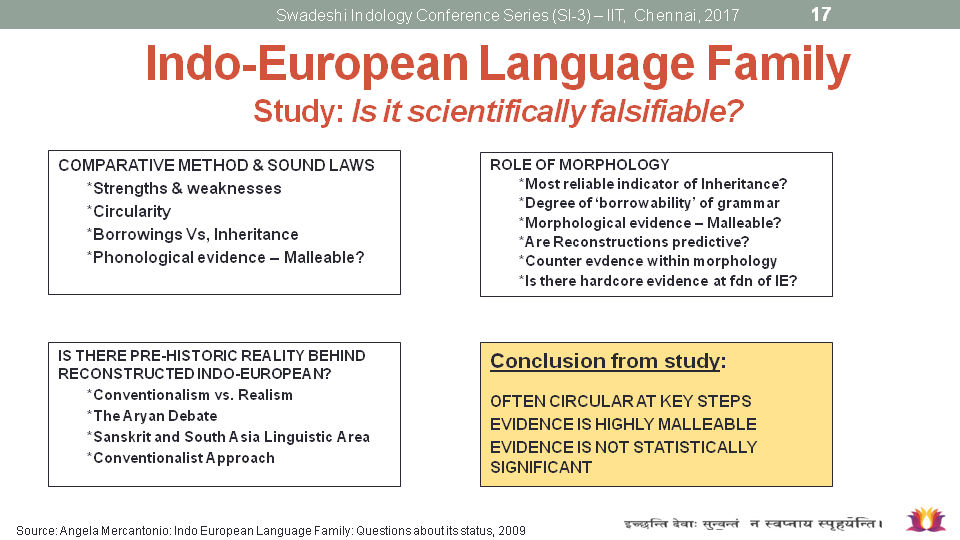
\includegraphics{"images/article-02/art02-fig01.jpg"}
\caption{Fig 1: Indo European Language family Problematized}
\end{figure}


\begin{figure}
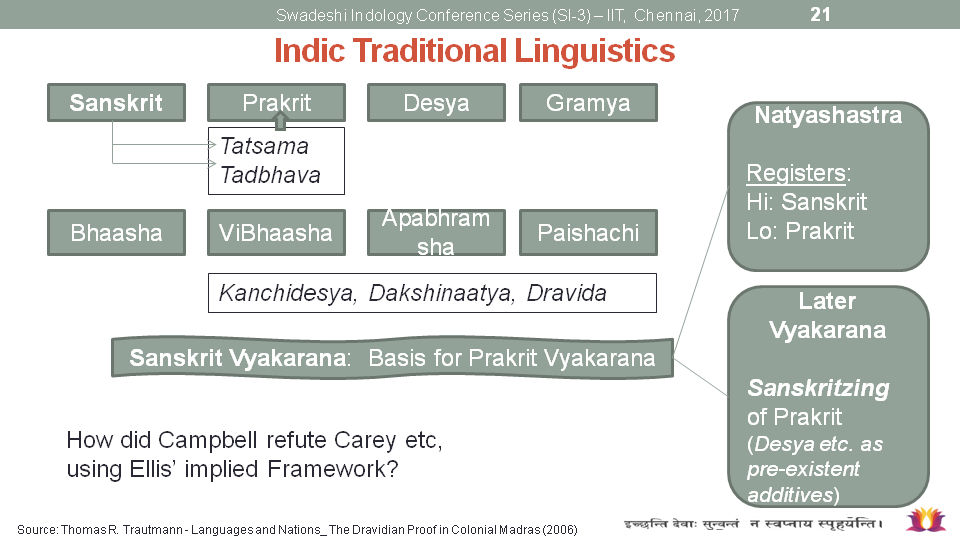
\includegraphics{"images/article-02/art02-fig02.jpg"}
\caption{Fig 2: Indic traditional linguistic basics}
\end{figure}


\begin{figure}
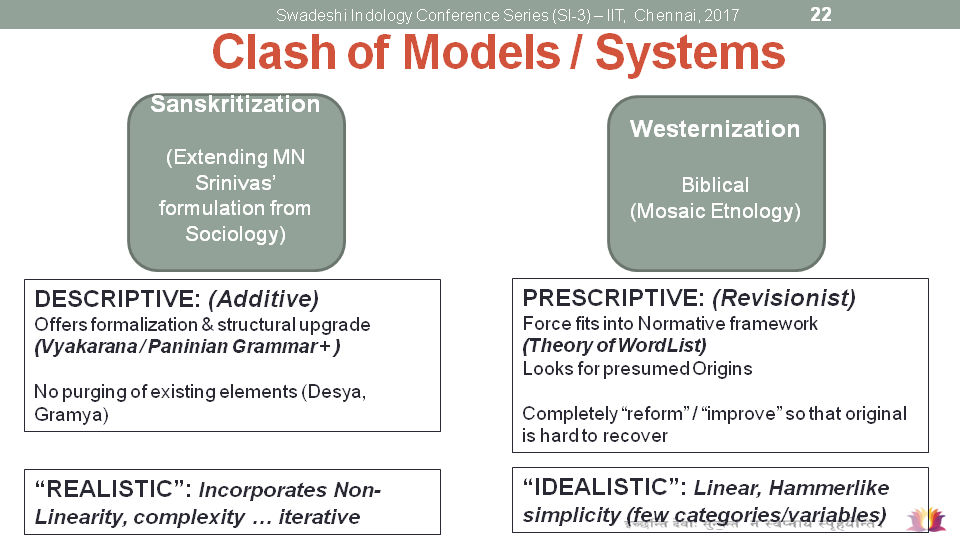
\includegraphics{"images/article-02/art02-fig03.jpg"}
\caption{Fig 3: Clash of models – Sanskritic vs. Western}
\end{figure}

This paper is based on, and can be seen in conjunction with, the published talks by the author (Joshi, Ravi 2017) and co-author (Harshavardhana, Yamuna 2017) at the recently concluded third Swadeshi Indology Conference.


\section*{Bibliography}

\begin{thebibliography}{99}
\bibitem{chap2-key01} Adluri, Vishwa P (2011). “Frame Narratives and Forked Beginnings: Or, How to Read the Ådiparvan”. \textit{Journal of Vaishnava Studies}, 19(2), 143-210.

 \bibitem{chap2-key02} Allchin, F. R. (1963). \textit{Neolithic cattle-keepers of south India: a study of the Deccan ashmounds} (No. 9). CUP Archive.

 \bibitem{chap2-key03} Ambedkar, B. R., (1949). \textit{Who were the Shudras?}

 \bibitem{chap2-key04} Baird, Robert D. et al., (1971) \textit{Indian and Far Eastern Religious Traditions}. New York: Harper \& Row

 \bibitem{chap2-key05} Bronkhorst, Johannes, (2003) “HINDUISM AND BUDDHISM”; (pp 327-330), entry in \textit{Gale Encyclopedia of Buddhism} (Ed.) Robert E. Buswell, Jr.

 \bibitem{chap2-key06} Chakrabarti, Dilip, (1997) \textit{Colonial Indology, Sociopolitics of the Ancient Indian Past}. New Delhi: Munshiram Manoharlal Publishers.

 \bibitem{chap2-key07} Coomaraswamy, Ananda. K. (1927). “The origin of the Buddha image”. \textit{The Art Bulletin}, 9(4), 287-328.

 \bibitem{chap2-key08} Datta, Amaresh, (1988) \textit{Encyclopaedia of Indian Literature, Volume 2}, Sahitya Akademi

 \bibitem{chap2-key09} Dharwadker, Vinay. (2002). “AK Ramanujan’s theory and practice of translation”. \textit{Post-colonial Translation: Theory and Practice}, 114-140.

 \bibitem{chap2-key10} Dharampal, Shri, \textit{Despoliation and Defaming of India–The Early Nineteenth Century, British Crusade}

 \bibitem{chap2-key11} Elst, Koenraad, (2017) \textit{The Tamil Veda}. Available at: http://www.pragyata.com/mag/the-tamil-veda-373

 \bibitem{chap2-key12} Fischer, Steven Roger, (1999) \textit{A History of Language}, The Netherlands: Reakton books

 \bibitem{chap2-key13} Foster, Arnold. (1973). General and Theoretical: Kings and Councillors: An Essay in the Comparative Anatomy of Human Society. AM HOCART. \textit{American Anthropologist}, 75(2), 403-404.

 \bibitem{chap2-key14} Frykenberg, Robert E, (2008) \textit{Christianity in India from beginnings to the present}. New York: Oxford University Press.

 \bibitem{chap2-key15} Hanneder, J. (2002). "On "The Death of Sanskrit"". Indo-Iranian Journal. Brill Academic Publishers.

 \bibitem{chap2-key16} Harper, Susan B. (2000). \textit{In the shadow of the Mahatma: Bishop VS Azariah and the travails of Christianity in British India}. Wm. B. Eerdmans Publishing.

 \bibitem{chap2-key17} Harper, Susan B. (1995). Ironies of indigenization: Some cultural repercussions of mission in South India. \textit{International Bulletin of Missionary Research}, 19(1), 13-20. Accessed at: https://pdfs.semanticscholar.org/6af8/f771af5073b49020d7de3280753c7ffbabf1.pdf

 \bibitem{chap2-key18} Hart, George L, (1976) \textit{The relation between Tamil and classical Sanskrit literature}. Wiesbaden: Harrassowitz. In \textit{A history of Indian literature: Vol. 10, Dravidian literature: Fasc. 2}

 \bibitem{chap2-key19} Hart, George L, (1987). Early Evidence for Caste in South India. \textit{Dimensions of Social Life: Essays in Honor of David G. Mandelbaum}, 48, 467. Version used here (preprint, cross checked with final) is available at: http://ww.tamilnation.co/caste/hart.pdf

 \bibitem{chap2-key20} Harshavardhana, Yamuna. (2017) \textit{Dravidianism with Language equaling Race -The third wheel in Tamil Sanskrit interactions}. Swadeshi Indology Conference 3, Track 2, Session 2: Modern Hinduphobia and the Dravidian Movement. Video available at: https://www.youtube.com/watch?v=mVOad19GbfY\&t=3084s

 \bibitem{chap2-key21} Hocart, Arthur M. (1970). \textit{Kings and councillors. Chicago}: The University of Chicago Press.

 \bibitem{chap2-key22} Inden, Ronald, (2000) \textit{Imagining India}. Bloomington: Indiana University Press

 \bibitem{chap2-key23} Ilakkuvanar, Maraimalai. Available at: https://www.academia.edu/11331219/George_L.Hart----_In_Defense_of_Classical_Tamil

 \bibitem{chap2-key24} Janson, Tore. (2002). \textit{Speak: A short history of languages}. Oxford: Oxford University Press.

 \bibitem{chap2-key25} Joshi, Ravi. (2017) \textit{Dravidianism with Language equaling Race -The third wheel in Tamil Sanskrit interactions}. Swadeshi Indology Conference 3, Track 2, Session 2: Modern Hinduphobia and the Dravidian Movement. Video available at: https://www.youtube.com/watch?v=mVOad19GbfY\&t=2535s

 \bibitem{chap2-key26} Kak, Subhash. (1994). On the classification of Indic languages. \textit{Annals of the Bhandarkar Oriental Research Institute}, 75(1/4), 185-195. Available at: http://www.ece.lsu.edu/kak/indic.pdf

 \bibitem{chap2-key27} Kak, Subhash. (1996). Indic language families and Indo-European. Yavanika, 6, 51-64. Available at: http://www.archaeologyonline.net/sites/default/files/imported/artifacts/Indic_Language_families.pdf

 \bibitem{chap2-key28} Krishnamurti, Bhadriraju, (2003) The Dravidian languages. Cambridge: Cambridge University Press.

 \bibitem{chap2-key29} Malhotra, R., \& Nīlakantan̲, A. (2011). \textit{Breaking India: Western Interventions in Dravidian and Dalit Faultlines}. New Delhi: Amaryllis.

 \bibitem{chap2-key30} Malhotra, Rajiv, (2013). \textit{Being different: An Indian challenge to western universalism}. New Delhi: HarperCollins India.

 \bibitem{chap2-key31} Mallikarjun, B. (2004). Indian multilingualism, language policy and the digital divide. \textit{Language in India}, 4(4), 109-113. Available at: http://www.ciillibrary.org:8000/ciil/repository/mallikarjun/m24.pdf

 \bibitem{chap2-key32} Mercantonio, Angela, (2009) \textit{The Indo European Language Family: Questions About Its Status}. Washington DC: Journal of Indo European Studies Monograph Series No. 55. Institute for the Study of Man, Inc.

 \bibitem{chap2-key33} Morrison, K. D., Lycett, M. T., \& Trivedi, M. (2016). Megaliths and memory: excavations at Kadebakele and the megaliths of Northern Karnataka. \textit{In Proceedings of the 20th Conference of the ‘European Association for South Asian Archaeology and Art} (Vol. 2, pp. 239-52).

 \bibitem{chap2-key34} Peterson, John K, (2010). Language contact in Jharkhand: Linguistic convergence between Munda and Indo-Aryan in eastern-central India. \textit{Himalayan Linguistics}, 9(2). Available at: https://cloudfront.escholarship.org/dist/prd/content/qt489929c1/qt489929c1.pdf

 \bibitem{chap2-key35} Peterson, John K, (2016) Fitting the pieces together – Towards a linguistic prehistory of eastern-central South Asia (and beyond). Available at: http://www.southasiabibliography.de/uploads/Peterson_Prehistory.pdf

 \bibitem{chap2-key36} Ramanujan, A K, (2005) \textit{Hymns for the Drowning}. Penguin Books India, 2005.

 \bibitem{chap2-key37} Ramasamy, Sumathi, \textit{The Quest for the Origins of Vedic Culture: The Indo-Aryan Migration Debate}

 \bibitem{chap2-key38} Rao, Ramakrishna, K. V. (2009), சங்க இலக்கியங்களில் ஆரியர்-திராவிடர், மதம் மற்றும் தத்துவங்களில் தென்னிந்தியாவின் பங்கு, திராவிடச் சான்றோர் பேரவை

 \bibitem{chap2-key39} Reddy, Srinivas, G (2011) \textit{The Āmuktamālyada of Kṛṣṇadevarāya: Language, Power \& Devotion in Sixteenth Century South India}. Berkeley: eScholarship, University of California. Phd Dissertation. Permalink: https://escholarship.org/uc/item/9v6585kp

 \bibitem{chap2-key40} Sanyal, S., \& Borgohain, R. (2013). Machine Translation Systems in India. \textit{Annals of the Faculty of Engineering Hunedoara-International Journal of Engineering}, 11(4). arXiv preprint arXiv:1304.7728 available at: https://arxiv.org/ftp/arxiv/papers/1304/1304.7728.pdf

 \bibitem{chap2-key41} Sjoberg, Andrée F. (1990) "The Dravidian Contribution to the Development of Indian Civilization: A Call for a Reassessment," Comparative Civilizations Review: Vol. 23: No. 23, Article 4. Available at: https://scholarsarchive.byu.edu/ccr/vol23/iss23/4

 \bibitem{chap2-key42} Srinivas, Narasimhachar, M. (1989). \textit{The cohesive role of Sanskritization and other essays}. Oxford University Press, USA.

 \bibitem{chap2-key43} Staal, Frits (1996) \textit{Ritual and Mantras: Rules without Meaning}. New Delhi: Motilal Banarasidass

 \bibitem{chap2-key44} Trautmann, Thomas R, (2006) \textit{Languages and nations: conversations in colonial South India}. Berkeley and Los Angeles: University of California Press

 \end{thebibliography}

